\documentclass[10pt]{amsart}
\usepackage[a4paper,margin=23mm]{geometry}
\usepackage{amsmath,amssymb,amsthm,mathtools,hyperref,graphicx,xspace,letltxmacro,xpatch}
\usepackage[english]{babel}
\newtheorem{theo}{Theorem}[section]
\newtheorem{lemm}[theo]{Lemma}\newtheorem{prop}[theo]{Proposition}\newtheorem{coro}[theo]{Corollary}\newtheorem{conj}[theo]{Conjecture}
\theoremstyle{definition}\newtheorem{defi}[theo]{Definition}\newtheorem{rema}[theo]{Remark}\newtheorem{exam}[theo]{Example}\newtheorem{exem}[theo]{Example}\newtheorem{nota}[theo]{Notation}
\newcommand{\ie}{i.e.}\newcommand{\eg}{e.g.}\newcommand{\resp}{resp.}\newcommand{\skpt}{\par\smallskip\noindent}
\emergencystretch=3em\pagestyle{plain}

\usepackage{dsfont}
\usepackage{amscd}



%%\AtBeginDocument{
%\newtheorem{myname}[cdrthm]{My beautiful theorem} }

\DeclareMathOperator{\GL}{GL}
\DeclareMathOperator{\SL}{SL}
\DeclareMathOperator{\id}{id}
\DeclareMathOperator{\Card}{Card}
\DeclareMathOperator{\Cov}{Cov}
\DeclareMathOperator{\Jac}{Jac}
\DeclareMathOperator{\Leb}{Leb}
\DeclareMathOperator{\Liouv}{Liouv}
\DeclareMathOperator{\Supp}{Supp}
\DeclareMathOperator{\Vect}{Vect}
\DeclareMathOperator{\VectSpan}{span}
\DeclareMathOperator{\Vol}{Vol}


\newcommand{\Z}{\mathbb{Z}}
\newcommand{\R}{\mathbb{R}}
\newcommand{\Cbb}{\mathbb{C}}
\newcommand{\B}{\mathbb{B}}
\newcommand{\Ebb}{\mathbb{E}}
\newcommand{\Lbb}{\mathbb{L}}
\newcommand{\Pbb}{\mathbb{P}}
\newcommand{\Sbb}{\mathbb{S}}
\newcommand{\Tbb}{\mathbb{T}}

\newcommand{\Acal}{\mathcal{A}}
\newcommand{\Bcal}{\mathcal{B}}
\newcommand{\Ccal}{\mathcal{C}}
\newcommand{\Fcal}{\mathcal{F}}
\newcommand{\Gcal}{\mathcal{G}}
\newcommand{\Hcal}{\mathcal{H}}
\newcommand{\Ical}{\mathcal{I}}
\newcommand{\Mcal}{\mathcal{M}}
\newcommand{\Ocal}{\mathcal{O}}
\newcommand{\Pcal}{\mathcal{P}}

\newcommand{\dd}{\;{\rm d}}
\newcommand{\de}{{\rm d}}
\newcommand{\norm}[2]{\left\| #1 \right\|_{#2}}

\newcommand*{\un}{\mathds{1}}



%%%%%%%%%%%%%%%%%%%%%%%%%%%%%%%%%%%%%%%%%%%%%%%%%%%%%%%%%%%%%%%%%%%
\graphicspath{{./figures/}}

\newcommand*{\mk}{\mkern -1mu}
\newcommand*{\Mk}{\mkern -2mu}
\newcommand*{\mK}{\mkern 1mu}
\newcommand*{\MK}{\mkern 2mu}

\hypersetup{urlcolor=purple, linkcolor=blue, citecolor=red}

\let\oldtilde\tilde
\renewcommand*{\tilde}[1]{\mathchoice{\widetilde{#1}}{\widetilde{#1}}{\oldtilde{#1}}{\oldtilde{#1}}}\let\oldhat\hat
\renewcommand*{\hat}[1]{\mathchoice{\widehat{#1}}{\widehat{#1}}{\oldhat{#1}}{\oldhat{#1}}}\let\oldforall\forall
\renewcommand*{\forall}{\mathrel{\oldforall}}
%%%%%%%%%%%%%%%%%%%%%%%%%%%%%%%%%%%%%%%%%%%%%%%%%%%%%%%%%%%

\title{Keplerian shear and invariant sigma-algebra for compatible affine torus-bundle flows}
\author{Thomine, Damien}
\date{doi:10.5802/ahl.42; CC BY 4.0}
\begin{document}
\maketitle
\noindent\textit{Editorial note.} Only selected author theorem counted; complete original mathematical body and bibliography preserved. Complete original vector PDF Forms retained; class-level theorem/remark environments supplied where needed.\par\medskip
\noindent\textit{Allowed standard prerequisites (editorial).}\begin{itemize}
\item Standard functional analysis, measure theory and the author-cited classical theorems. Standard prior results stay cited; complete source-local proofs and definitions retained.
\end{itemize}\medskip

\section{Introduction}

When a celestial body is orbiting circularily around another, Kepler's third law asserts that the period of the orbit is proportional to the radius of the orbit at the power $3/2$: closer bodies complete their orbits faster. When one considers bodies whose size is non-negligible with respect to the radius of the orbit, this difference of orbital periods induces a shearing effect, called Keplerian shear~\cite{Tiscareno:2012}. Keplerian shear is most notable in planetary rings, for instance Saturn's. As a consequence, any large-scale heterogeneity of the rings is wrapped around the rings, until -- for large enough times -- it equidistributes angularly (see Figure~\ref{fig:Saturne}): Keplerian shear explains the radial symmetry of large planetary rings.

\begin{figure}[h!]
\vspace{1cm}
\centering
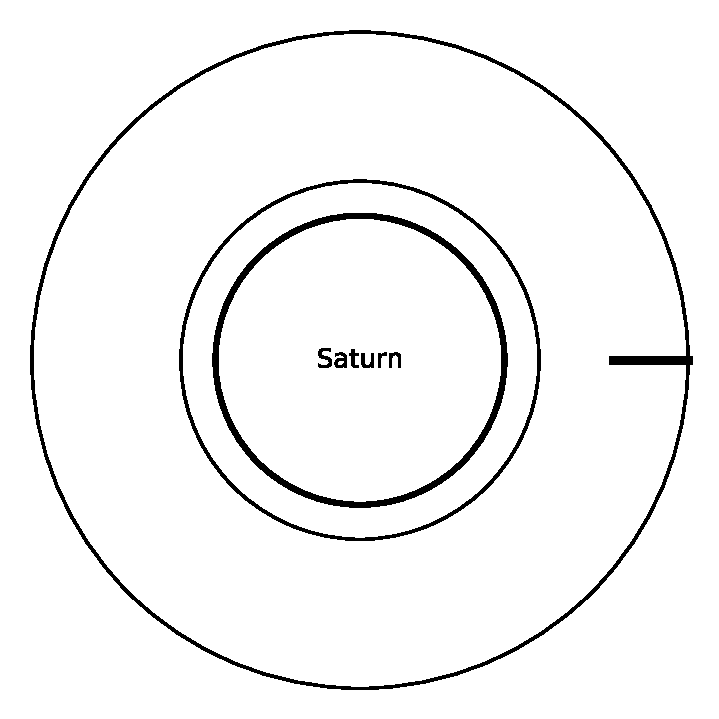
\includegraphics[scale=0.4]{./Saturn_0h.pdf}
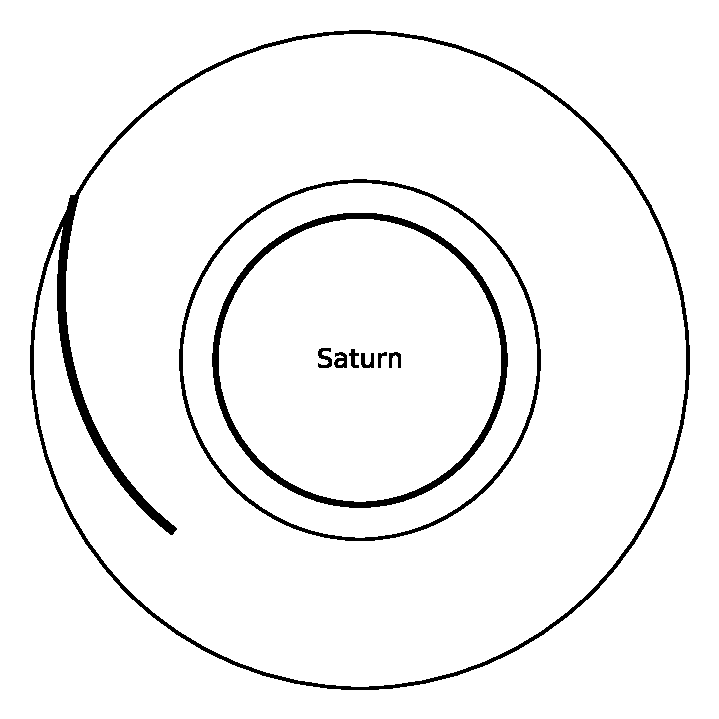
\includegraphics[scale=0.4]{./Saturn_6h.pdf}
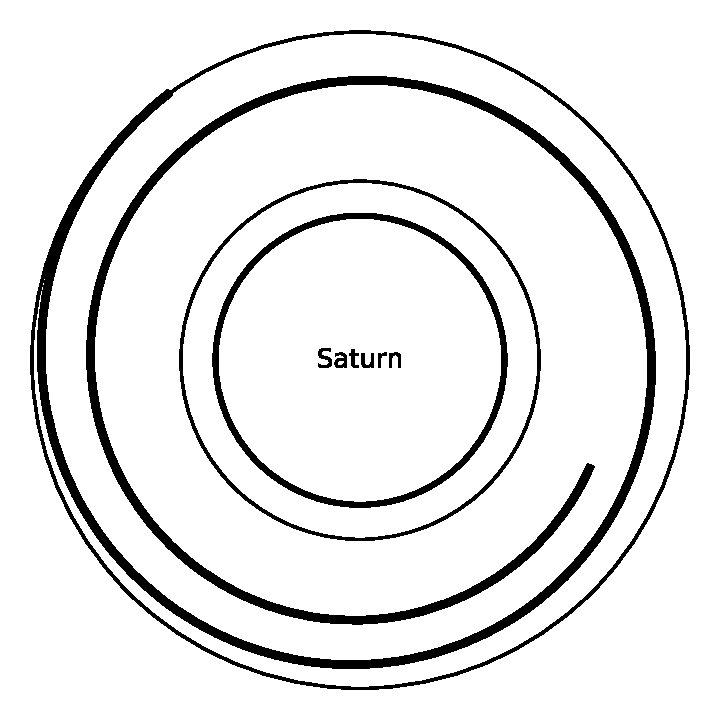
\includegraphics[scale=0.4]{./Saturn_48h.pdf}
\caption{Equirepartition of a cloud of dust in Saturn's rings. On the left: the cloud (thick black line) at initial time. In the middle: the same cloud, after 6 hours. On the right: the same cloud, after 48 hours.}\label{fig:Saturne}
\end{figure}

Keplerian shear is a more general feature of many integrable Hamiltonian dynamical systems. Using action-angle coordinates, the phase space is foliated by invariant Lagrangian tori, and the dynamics of a point belonging to the phase space is conjugate to a translation on one of these tori. Provided that the translations on the Lagrangian tori are (in some sense) asynchronous, the dynamics shear the transversals to the invariant tori, so that in large time, densities equidistribute along the tori. In the case of planetary rings, the invariant tori are orbits of given radius, and the asynchronicity comes from the variation of the orbital period: we recover classical Keplerian shear. Other systems with Keplerian shear are the geodesic flow on a flat torus (see Figure~\ref{fig:Tore}), or the dynamics of a ball bouncing in a square box.

\begin{figure}[h!]
\vspace{1cm}
\centering
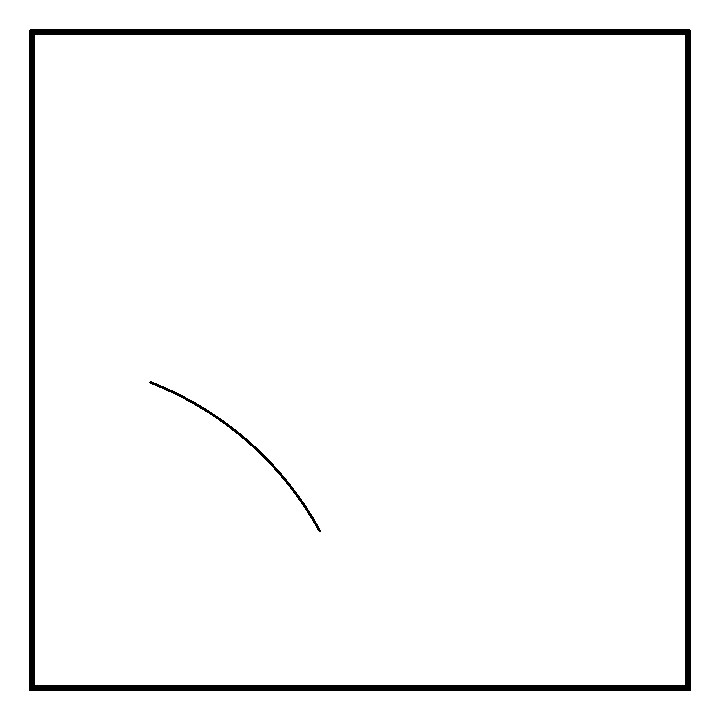
\includegraphics[scale=0.4]{./Torus_0_5.pdf}
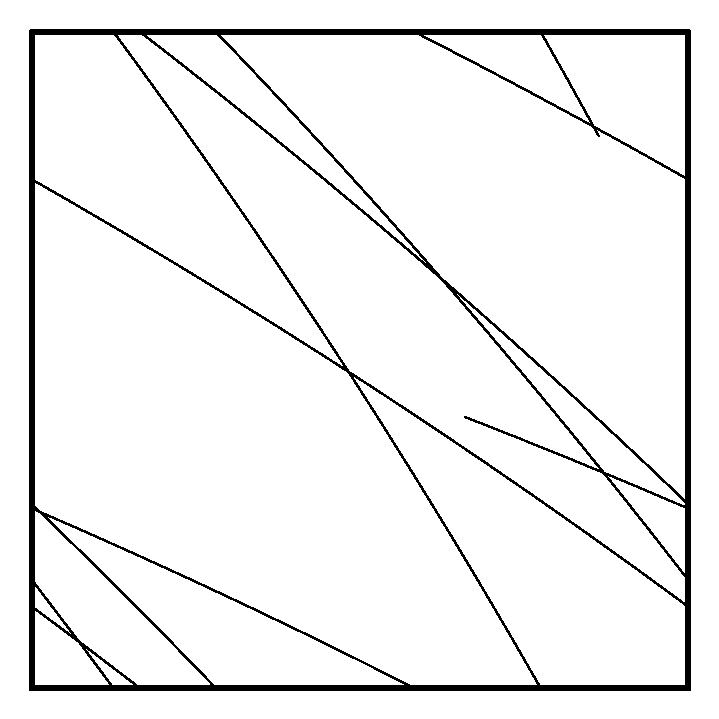
\includegraphics[scale=0.4]{./Torus_10.pdf}
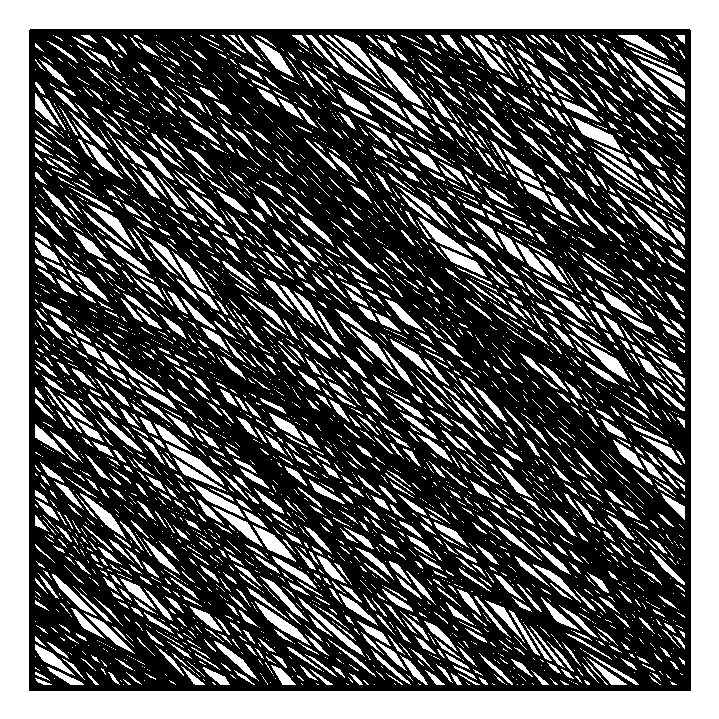
\includegraphics[scale=0.4]{./Torus_500.pdf}
\caption{Propagation of a wavefront at unit speed in a unit square torus. The wave starts from the corner, and propagates at unit speed. From left to right: the wavefront at times $0.5$, then $10$ and $500$ respectively.}\label{fig:Tore}
\end{figure}

%%\smallskip

In this article, we frame Keplerian shear in the more general context of ergodic theory, as a conditional version of the notion of strong mixing.

\begin{defi}[Keplerian shear]%%\quad
A dynamical system $(\Omega, \mu, (g_t)_{t \in \R})$ which preserves a probability measure is said to exhibit
\emph{Keplerian shear} if, for all\linebreak$f \in \Lbb^2 (\Omega, \mu)$,
\begin{equation}\label{eq:DefinitionKeplerianShear}
\lim_{t \to + \infty} f \circ g_t = \Ebb_\mu (f | \Ical),
\end{equation}
where $\Ical$ is the invariant $\sigma$-algebra and the convergence is for the weak topology on $\Lbb^2 (\Omega, \mu)$.
\end{defi}


Recall that a system $(\Omega, \mu, (g_t)_{t \in \R})$ is mixing if and only if, for any function $f \in \Lbb^2 (\Omega, \mu)$,
\[
\lim_{t \to + \infty} f \circ g_t = \int_\Omega f \dd \mu = \Ebb_\mu (f),
\]
where the limit is taken in the weak topology on $\Lbb^2 (\Omega, \mu)$, so a system $(\Omega, \mu, (g_t)_{t \in \R})$ is mixing if and only if it is ergodic and exhibits Keplerian shear. As such, Keplerian shear is a conditional version of the notion of strong mixing. Informally, if the system restricted to its invariant subsets is mixing, then $(\Omega, \mu, (g_t)_{t \in \R})$ has Keplerian shear. The interesting examples occur when these restrictions are ergodic, but not mixing: that is the case, for instance, of translation flows on a torus.

%%\smallskip

In this article, we give a criterion ensuring Keplerian shear for a large class of such systems; for instance, one of our result is:

\begin{prop}[Corollary of Theorem~\ref{thm:ClassiquePrincipal} and Proposition~\ref{prop:BaireGenericite}]\ \\*[0.10em]
Let $M$ be a Riemannian manifold, $d \geq 1$ and $k \in [1, \infty]$. Let $v \in \Ccal^k (M, \R^d)$, and put $g_t (x,y) := (x, y+tv(x))$ for $(x,y)\in M \times \Tbb^d$. If:
\[
\Vol_M (\de \langle \xi, v \rangle = 0) = 0 \quad \forall \xi \in \Z^d \setminus \{0\},
\]
then the invariant $\sigma$-algebra $\Ical$ is (up to completion) $\Bcal (M) \otimes \{0, \Tbb^d\}$, and the\linebreak dynamical system $(M \times \Tbb^d, \Vol_M \otimes \Leb_{\Tbb^d}, (g_t))$ exhibits Keplerian shear. Moreover, the above criterion is satisfied for a generic $v \in \Ccal^k (M, \R^d)$.
\end{prop}

We also study the rate of decay of conditional covariance for the geodesic flow on $T^1 \Tbb^d$, and give non-trivial examples of non-Hamiltonian systems with Keplerian shear.

%%\smallskip

Keplerian shear for the geodesic flow on the flat torus is related to two famous problems. The first is Landau's damping for plasma dynamics on a torus (see\linebreak Landau's article~\cite{Landau:1946}, and~\cite[Theorem~3.1]{MouhotVillani:2011} for a version which follows closely our formalism), where the effect is qualitatively similar, although the underlying mechanism is different. The second is Gauss's circle problem, which consists in counting integral points in a large disc; we shall discuss it in Sub-subsection~\ref{subsubsec:Gauss}. The methods used to tackle these problems are either through Fourier transform (e.g. for Landau damping), or with a big arc/small arc decomposition (typical for Gauss's circle problem). While both methods work in our setting, we shall only use the Fourier transform.

%%\smallskip

In the context of ergodic theory, a notion closely related with Keplerian shear was used independently by F.~Maucourant~\cite{Maucourant:2016} to prove that the some hyperbolic actions on $(\R^d \rtimes SL_d (\R))_{/(\Z^d \rtimes SL_d (\Z))}$ are ergodic for a large class of measures. The presentation in~\cite{Maucourant:2016} is however very different, as the phenomenon -- named \emph{asynchronicity} -- is described as a version of unique ergodicity for measures with prescribed marginals.


\subsection{Organization of the article}

Section~\ref{sec:ProprietesFondamentales} gives general results on the notion of Keplerian shear (including equivalences between distinct definitions), and gives us some tools to use for the remainder of the article.

%%\smallskip

Section~\ref{sec:FibreBundle} deals with a first family of systems which may exhibit Keplerian shear: fibrations by tori, where the flow acts by translation on each torus. Using action-angle coordinates, this family includes integrable Hamiltonian flows. We give an explicit criterion ensuring Keplerian shear, check that it is $\Ccal^r$-generic ($r \geq 1$) and satisfied for some explicit systems, then give rates of convergence for the geodesic flow on $T^1 \Tbb^n$. We also detail the link between Keplerian shear and the unique ergodicity as investigated in~\cite{Maucourant:2016}.

%%\smallskip

Section~\ref{sec:StretchedBirkhoff} deals with another family of dynamical systems (roughly, flows with a change of time), which includes many non-Hamiltonian examples, and uses a different mechanism to ensure Keplerian shear.

%%smallskip

The shorter Section~\ref{sec:SansMelange} gives examples of systems without Keplerian shear.


\subsection{A note on the terminology}

Given that Keplerian shear is a conditional version of the notion mixing, one could want to use a terminology such as \emph{conditional (strong) mixing}. For this article, we prefer to eschew this option, and to keep the name of Keplerian shear; indeed, we think that otherwise the name of conditional (strong) mixing would be overloaded.

%%\smallskip

In probability theory, there are already multiple notions of conditional mixing; compare for instance~\cite{Rao:2009} (where it refers to conditional $\alpha$-mixing) and~\cite{KacemLoiselMaumeDeschamps:2016}, among others.

%%\smallskip

More worryingly, in ergodic theory, the notion of conditionally weakly mixing systems is well-established (see e.g.~\cite{Tao:2008}), but if one where to conceive a notion of conditional strong mixing along this line, the resulting notion would be stronger than Keplerian shear, essentially requiring that almost every subsystem in its ergodic decomposition be mixing.


\subsection{Open problems}

We sum up here some further leads which seem worth pursuing.

%%\smallskip

The setting of Section~\ref{sec:FibreBundle} covers integrable Hamiltonian systems. However, it requires some regularity, and in particular it does not cover singular systems. A conjecture by Boshernitzan asserts that given a compact translation surface $S$, the geodesic flow on $(T^1 S, \Liouv)$ exhibits Keplerian shear. This question, mentioned as \emph{illumination by circles}, also appears in~\cite{Monteil:2005}, and admits a partial answer by J.~Chaika and P.~Hubert~\cite{ChaikaHubert:2015}, where the convergence of $\Ebb (\Cov_t (f, h|\Ical))$ to zero, with:
\[
\Cov_t (f, h|\Ical) := \Ebb (f \cdot h \circ g_t|\Ical) - \Ebb (f |\Ical)\Ebb (h|\Ical),
\]
is shown along a density $1$ subsequence for all continuous observables $f$ and $h$\footnote{Technically, J.~Chaika and P.~Hubert show the convergence only for observables which do not depend on the direction, but a straightforward generalization and a diagonal argument yield the general case.}.

%%\smallskip

In Subsection~\ref{subsec:Speed}, we investigate the speed of Keplerian shear for the geodesic flow on $T^1 \Tbb^n$. The problem is simplified by the particularities of the geometry of the sphere, more precisely the fact that its principal curvatures do not vanish. What would the speed of convergence be if the curvature vanishes (e.g.~in a topologically or measure-theoretically generic setting)?

%%\smallskip

Finally, while the settings of Sections~\ref{sec:FibreBundle} and~\ref{sec:StretchedBirkhoff} are distinct and Keplerian shear arises from different mechanisms, a more general structure (spaces fibrated by suspension tori) mixes the difficulties of both. However, even a description of the invariant $\sigma$-algebra $\Ical$ is not obvious at this level of generality.



\section{General properties of Keplerian shear}\label{sec:ProprietesFondamentales}

The following Lemma~\ref{lem:LemmeAnalyseFonctionnelle} from basic functional analysis is quite useful to prove the ergodicity and mixing of any given dynamical system, and will be instrumental in the remainder of our article.

\begin{lemm}\label{lem:LemmeAnalyseFonctionnelle}

Let $\B$ be a Banach space. Let $(T_t)_{t \geq 0}$ be a family of operators on $\B$, such that $\sup_{t \in \R_+} \norm{T_t}{\B \to \B} < + \infty$. Let $T$ be an operator on $\B$.

Let $E$ and $E^*$ be subsets of $\B$ and $\B^*$ respectively, whose span is dense in their respective space. Assume that, for all $f \in E$ and $g \in E^*$,
\begin{equation}\label{eq:ConvergenceFaible}
\lim_{t \to + \infty} \langle g, T_t f \rangle = \langle g, T f \rangle.
\end{equation}

Then $(T_t f)_{t \geq 0}$ converges weakly to $T f$ for all $f \in \B$.
\end{lemm}


\begin{proof}%%\quad
By bilinearity, Equation~\eqref{eq:ConvergenceFaible} holds for all $f \in \VectSpan(E)$ and $g \in \VectSpan(E^*)$.
Since $\sup_{t \in \R_+} \norm{T_t}{\B \to \B} < + \infty$, the family of functions $T_t : \B^* \times \B \to \Cbb$ is locally equicontinuous, and by the remark above, it converges to $T$ on a dense subset. Hence, the convergence of Equation~\eqref{eq:ConvergenceFaible} holds for all $f \in \B$ and $g \in \B^*$.
\end{proof}



When we use Lemma~\ref{lem:LemmeAnalyseFonctionnelle}, the operator $T_t$ shall correspond to the composition by the flow $g_t$ at time $t$, and the operator $T$ to the projection $f \mapsto \Ebb (f | \Ical)$; if $\B = \Lbb^2$, then $\Ebb (f | \Ical)$ is actually the orthogonal projection of $f$ onto the closed subspace of $\Ical$-measurable square-integrable functions. Since the flow is assumed to preserve the measure, for all $t \geq 0$ and all $p \in [1, + \infty]$, the operator $T_t$ acting on $\Lbb^p (\Omega, \mu)$ is unitary. Lemma~\ref{lem:LemmeAnalyseFonctionnelle} implies that to prove the Keplerian shear in one of those Banach space $\B$ (potentially different from $\Lbb^2$), it is enough to restrict ourselves to subsets $E$ of $\B$ and $E^*$ of $\B^*$ whose linear span is dense. As a first consequence, in the definition of Keplerian shear, one may replace $\Lbb^2$ by $\Lbb^p$ for any $p \in [1, +\infty)$:


\begin{prop}
Let $(\Omega, \mu, (g_t)_{t \in \R})$ be a flow which preserves a probability measure. Let $\Ical$ be the invariant $\sigma$-algebra of the system. Then there is equivalence between:
\begin{itemize}
\item There exists $p \in [1, + \infty)$ such that, for all $f \in \Lbb^p (\Omega, \mu)$, we have $f \circ g_t \to \Ebb (f | \Ical)$ weakly in $\Lbb^p$.
\item The system exhibits Keplerian shear.
\item For all $p \in [1, + \infty)$, for all $f \in \Lbb^p (\Omega, \mu)$, we have $f \circ g_t \to \Ebb (f | \Ical)$ weakly in~$\Lbb^p$.
\end{itemize}
\end{prop}

\begin{proof}
We only prove the non-trivial implication. Let $p \in [1, + \infty)$. Assume such that, for all $f \in \Lbb^p (\Omega, \mu)$, we have $f \circ g_t \to \Ebb (f | \Ical)$ weakly in $\Lbb^p$. Then, since $\Lbb^\infty \subset \Lbb^p \cap (\Lbb^p)^*$, for all $f_1$ and $f_2$ in $\Lbb^\infty$,
\[
\lim_{t \to + \infty} \Ebb(f_1 \cdot f_2 \circ g_t) = \langle f_1, \Ebb (f_2 | \Ical)).
\]
Let $q \in [1, + \infty)$. Since $\Lbb^\infty$ is dense in both $\Lbb^q$ and $(\Lbb^q)^*$, by Lemma~\ref{lem:LemmeAnalyseFonctionnelle}, the convergence above occurs for all $f_1$ and $f_2$ in $\Lbb^q$ and $(\Lbb^q)^*$ respectively.
\end{proof}
\goodbreak


A second consequence is that Keplerian shear is not only a property of the invariant measure $\mu$, but of the class of $\mu$.


\begin{prop}\label{prop:MesuresAbsContinues}

Let $(\Omega, \mu, (g_t)_{t \in \R})$ be a flow which preserves a probability measure and exhibits Keplerian shear. Let $\nu \ll \mu$ be a probability measure which is also $(g_t)$-invariant. Then $(\Omega, \nu, (g_t)_{t \in \R})$ also exhibits Keplerian shear.
\end{prop}


\begin{proof}
Let $(\Omega, \mu, (g_t)_{t \in \R})$ and $\nu$ be as in assumptions of the proposition. Let $h := \de \nu / \de \mu$. Since $\nu$ is $(g_t)$-invariant, the function $h$ is $\Ical$-measurable.

%%\smallskip

Let $f_1$ be in $\Lbb^\infty (\Omega, \mu)$ be such that $f_1h \in \Lbb^2 (\Omega, \mu)$, and let $f_2 \in \Lbb^\infty (\Omega, \mu)$. Recall that the conditional expectation $\Ebb_\mu (f_2 | \Ical)$ is the unique $\Ical$-measurable function in $\Lbb^2 (\Omega, \mu)$ such that, for all $\Ical$-measurable and bounded $k$,
\[
\Ebb_\mu (\Ebb_\mu(k f_2 | \Ical)) = \Ebb_\mu (k \Ebb_\mu(f_2 | \Ical)).
\]
Given a $\Ical$-measurable and bounded function $k$ and since $h$ is $\Ical$-measurable,
\begin{align*}
\Ebb_\nu (\Ebb_\mu(k f_2 | \Ical)) & = \Ebb_\mu (h \Ebb_\mu(k f_2 | \Ical)) = \Ebb_\mu (\Ebb_\mu(hk f_2 | \Ical)) \\
& = \Ebb_\mu (hk \Ebb_\mu(f_2 | \Ical)) = \Ebb_\nu (k \Ebb_\mu(f_2 | \Ical)).
\end{align*}
By the previous characterization of the conditional expectation, $\nu$-almost surely, $\Ebb_\nu(f_2 | \Ical) = \Ebb_\mu(f_2 | \Ical)$. Let $t \geq 0$. Then:
\[
\Ebb_\nu (f_1 \cdot f_2 \circ g_t) = \Ebb_\mu ((f_1h) \cdot f_2\circ g_t).
\]
Since the initial system is assumed to have Keplerian shear, $f \in \Lbb^\infty (\Omega, \mu)$ and $gh \in \Lbb^\infty (\Omega, \mu)$, we get:
\[
\lim_{t \to + \infty} \Ebb_\nu (f_1 \cdot f_2 \circ g_t) = \Ebb_\mu (f_1h\Ebb_\mu (f_2 | \Ical)) = \Ebb_\nu (f_1 \Ebb_\nu (f_2 | \Ical)).
\]
The canonical projection $\Lbb^\infty (\Omega, \mu) \to \Lbb^\infty (\Omega, \nu)$ is surjective, so its image is dense in $\Lbb^2 (\Omega, \nu)$. The image of the set of functions $f_1 \in \Lbb^\infty (\Omega, \mu)$ such that $f_1h \in \Lbb^2 (\Omega, \mu)$ by this projection is also dense in $\Lbb^2 (\Omega, \nu)$. We use Lemma~\ref{lem:LemmeAnalyseFonctionnelle} to conclude.
\end{proof}


The last Lemma~\ref{lem:LemmeAnalyseFonctionnelle} asserts that, in the definition of Keplerian shear, the limit object $\Ebb_\mu (f | \Ical)$ cannot be meaningfully modified.


\begin{prop}
%%\quad
Let $(\Omega, \mu, (g_t)_{t \in \R})$ be a flow which preserves a probability measure. Let $f, h \in \Lbb^2 (\Omega, \mu)$.
%%\smallskip
If $(f \circ g_t)_{t \in \R}$ converges weakly to $h$, then $h = \Ebb_\mu (f | \Ical)$.
\end{prop}


\begin{proof}
Let $f_2 \in \Lbb^2 (\Omega, \mu)$. Our hypotheses imply that $\lim_{t \to + \infty} \Ebb_\mu (f_2 \cdot f \circ g_t)\linebreak= \Ebb_\mu (f_2 h)$. In addition, the function $t \to \Ebb_\mu (f_2 \cdot f \circ g_t)$ is measurable and bounded. By taking the Cesàro average, we get:
\[
\lim_{t \to + \infty} \Ebb_\mu \left(\frac{f_2}{t} \int_0^t f \circ g_s \dd s \right) = \lim_{t \to + \infty} \frac{1}{t} \int_0^t \Ebb_\mu (f_2 \cdot f \circ g_s) \dd s = \Ebb_\mu (f_2 h).
\]
On the other hand, by von Neumann's ergodic theorem,
\[
\lim_{t \to + \infty} \Ebb_\mu \left(\frac{f_2}{t} \int_0^t f \circ g_s \dd s \right) = \Ebb_\mu (f_2 \Ebb_\mu (f | \Ical)).
\]
Since this holds for all $f_2 \in \Lbb^2$, we have $h = \Ebb_\mu (f | \Ical)$.
\end{proof}



\begin{rema}
%%\quad

In most examples in this article, $\Omega = M \times A$ is a product space, the invariant $\sigma$-algebra is the Borel $\sigma$-algebra of $M$, and $\mu = \mu_M \otimes \mu_A$ is the product of two probability measures. In this situation, the conditional expectation admits a simple expression:
\[
\Ebb_\mu (f | \Ical) (x) = \int_{\{x\} \times A} f(x,y) \dd \mu_A (y).
\]
Note that the value of $\Ebb_\mu (f | \Ical)$ does not depend on $\mu_M$. For instance, for planetary rings in polar coordinates, the state space is $[a,b] \times \Tbb_1$, the flow preserves each circle $\{r\} \times \Tbb^1$, the invariant $\sigma$-algebra $\Ical$ is the $\sigma$-algebra of radially symmetric measurable sets, and for any probability measure $\mu = \mu_{[a,b]} \otimes \Leb$:
\[
\Ebb_\mu (f | \Ical) (r) = \frac{1}{2\pi} \int_0^{2 \pi} f(r,\theta) \dd \theta.
\]
\end{rema}


\section{Affine tori bundles}\label{sec:FibreBundle}

\subsection{Setting and main theorem}\label{subsec:TheoremePrincipal}


We generalize our introductory examples to a class of flows on fibre bundles by tori which leave the basis invariant. More specifically, the spaces on which we work are the following:

\begin{defi}[Affine tori bundles]%%\quad
An affine tori bundle is a $\Ccal^1$ manifold $\Omega$ which is a fiber bundle by $d$-dimensional tori, with group structure $\Tbb^d \rtimes \GL_d (\Z)$. In other words, there exist:
\begin{itemize}
\item two integers $n$, $d \geq 1$;
\item a $n$-dimensional $\Ccal^1$ real manifold $M$;
\item a $\Ccal^1$ projection $\pi : \ \Omega \to M$;
\item a maximal atlas $\Acal$ on $M$,
\end{itemize}
such that, for all $U \in \Acal$, we have a diffeomorphism $\psi_U : \pi^{-1} (U) \to U \times \Tbb^d$ such that $\pi_1 \circ \psi_U = \pi$, and the change of charts are given by:
\[
\psi_V \circ \psi_U^{-1} : 
\begin{cases}
(U \cap V) \times \Tbb^d & \to (U \cap V) \times \Tbb^d \\
(x,y) & \mapsto (x, \alpha_{U, V} (x) + A_{U, V} (y))
\end{cases}
\]
where $\alpha_{U,V}$ is $\Ccal^1$ and $A_{U, V} \in \GL_d (\Z)$.
\end{defi}


The notions of ``subset of zero Lebesgue measure'' or ``subset of full Lebesgue measure'' are well-defined on $\Ccal^1$ manifolds (as they are invariant by diffeomorphisms), and thus so is the notion of ``probability measure absolutely continuous with respect to the Lebesgue measure''. We will abuse notations and write $\Leb (A) = 0$ for a measurable subset of zero Lebesgue measure $A$, and $\mu \ll \Leb$ for an absolutely continuous measure.


\begin{defi}[Compatible flows]%%\quad
Let $\Omega$ be an affine tori bundle. A flow $(g_t)_{t \in \R}$ on $\Omega$ is said to be \emph{compatible on a chart} $\psi_U : \ \pi^{-1} (U) \to U \times \Tbb^d$ if there exists $v_{\psi_U} \in \Ccal^1 (U, \R^d)$ such that, for all $t \in \R$,
\[
\psi_U \circ g_t \circ \psi_U^{-1} (x,y) = (x, y + t v_\psi (x)).
\]

A $\sigma$-finite measure $\mu$ on $\Omega$ is said to be \emph{compatible on a chart} $\psi_U : \ \pi^{-1} (U) \to U \times \Tbb^d$ if $\psi_{U,*} \mu_{|\pi^{-1} (U)} = (\pi_* \mu)_{|U} \otimes \Leb_{\Tbb^d}$.

%%\smallskip

A flow or a measure is said to be \emph{compatible} if it is compatible on all charts.
\end{defi}


A compatible measure is always invariant under a compatible flow. In addition, this notion behaves well with respect to the affine structure on the manifolds we work with. If a flow or a measure is compatible on some chart $\psi_U: U \cap V \to \pi (U \cap V) \times \Tbb^d$ and if $\psi_{U,V}$ is a change of charts, then the flow or the measure is compatible on the chart $\psi_{V|U \cap V}: U \cap V \to \pi (U \cap V) \times \Tbb^d$.

%%\smallskip

In what follows, we shall work mostly with absolutely continuous measures. In this case, what happens on a subset of zero Lebesgue measure does not matter: the assumption that $M$ be a manifold can be weakened to account for singularities or boundaries.

%%\smallskip

In light of the previous paragraph, the introduction of the structure group $\Tbb^d \rtimes \GL_d (\Z)$ might look gratuitous: one can always cut out the manifold $M$ along a set of zero Lebesgue measure to get a disjoint union of simply connected domains, on which there is no holonomy. However, this structure appears naturally in many\linebreak examples. For instance, for all $n \geq 1$, we can work with the geodesic flow on $T \Sbb_n$: if we ignore the set of null tangent vectors, which is negligible, we get a fibre bundle over\linebreak$\R_+^* \times \widetilde{Gr} (2, n+1)$ with fibre $\Sbb_1$. With the same adaptation, our setting also includes billiards in ellipsoids or the geodesic flow on ellipsoids (see C.~Jacobi~\cite{Jacobi:1866} for the geodesic flow on ellipsoids, J.~Moser~\cite{Moser:1978} for similar examples, and S.~Tabachnikov~\cite{Tabachnikov:2002} for the relation between the geodesic flow and the billiard). Let us also mention the study of the geodesic flow on $(\R^d \rtimes \SL_d (\R))_{/ \Z^d \rtimes\SL_d (\Z)}$ done by F.~Maucourant~\cite{Maucourant:2016}, in which the same structure appears.

%%\smallskip

Another important remark is that, when we change charts from chart $U$ to chart $V$, we have $v_{\psi_V | U \cap V} = A_{U, V} v_{\psi_U | U \cap V}$. So, while there is in general no well-defined function $v : \ M \to \R^d$ which gives the direction of the flow, the set of functions $\{x \mapsto \langle \xi, v(x) \rangle\}_{\xi \in \Z^d - \{0\}}$ is well-defined.

%%\smallskip

We are now ready to state our main Theorem~\ref{thm:ClassiquePrincipal}.


\begin{theo}\label{thm:ClassiquePrincipal}

Let $\pi: \Omega \to M$ be an affine $d$-dimensional tori bundle over a manifold $M$. Let $(g_t)_{t \in \R}$ be a compatible flow, and $\mu$ be an absolutely continuous compatible probability measure.

%%\smallskip

If $\Leb \left(\bigcup_{\xi \in \Z^d - \{0\}} \{ \de \langle \xi, v \rangle = 0\}\right) = 0$ on $M$, then the invariant $\sigma$-algebra $\Ical$ is (up to completion) $\pi^{-1} \Bcal (M)$, and the dynamical system $(\Omega, \mu, (g_t))$ exhibits Keplerian~shear.
\end{theo}



\begin{proof}
Assume that $\Leb \left(\bigcup_{\xi \in \Z^d - \{0\}} \{ \de \langle \xi, v \rangle = 0\}\right) = 0$. Then $\Leb \big(\bigcup_{\xi \in \Z^d - \{0\}} \{ \langle \xi,\linebreak v \rangle= 0\}\big)= 0$, so $(g_t (x,y))_{t \in \R}$ equidistributes in $\{x\} \times \Tbb^d$ for Lebesgue-almost every $x$. Hence, up to completion by the measure $\mu$, the invariant $\sigma$-algebra of the flow is $\Ical := \pi^* \Bcal_M$, where $\Bcal_M$ is the Borel $\sigma$-algebra of $M$.

%%\smallskip

Our goal is to find a family of observables which is large enough to generate a dense subset of $\Lbb^2 (\Omega, \mu)$, and specific enough to make our computations manageable. Roughly, we choose a specific frequency in the direction of the torus $\Tbb^d$. Under the hypothesis of the Theorem~\ref{thm:ClassiquePrincipal}, we can rectify the differential form $\langle \xi, v \rangle$ so that it has a very simple expression. Then we choose observables which split into an observable $a$ in the direction of $\langle \xi, v \rangle$, and another observable $b$ in the direction of the kernel. The later observable $b$ does not see the shearing at all, so the shearing only affects $a$.

%%\smallskip

Let $(U_i, \varphi_i)_{i \in I}$ be a countable cover of $M$ by disjoint open charts\footnote{The goal of this first decomposition is only to get well-defined speed functions $v_{\psi_i}$, and can be bypassed if the fibre bundle is trivial.}, up to a Lebesgue-negligible set, with $\varphi_i : U_i
\to W_i \subset \R^n$. Let $\psi_i : \pi^{-1} (U_i) \to U_i \times \Tbb^d$ be a family of trivializing charts for $\Omega$, and let $v_i := v_{\psi_i}$.

%%\smallskip

For $\xi \in \Z^d \setminus \{0\}$, let $V_i^\xi := V_i \cap \{ \de \langle \xi, v_i \rangle = 0\}$. Using the local normal form of submersions, we can find a finite or countable family $(V_{ij}^\xi)_{j \in J(i,\xi)}$ of open sets which are pairwise disjoint, cover $V_i^\xi$ up to a Lebesgue-negligible set, and with charts $\varphi_{ij}^\xi : V_{ij}^\xi \to W_{ij}^\xi \subset \R^n$ such that $\langle \xi, v_i \rangle \circ \varphi_{ij}^{\xi,-1} (x) = x_1$. For $\xi=0$, we choose $J(i,\xi)$ to be a singleton and take $V_{ij}^0:=V_i$.

%%\smallskip

Given a point $p \in \R^n$, we write $p_x$ its first coordinate in $\R^n$, and $p_y$ for its remaining $n-1$ coordinates in $\R^n$. Given a point $p \in M \times \Tbb^d$, we write $p_z$ for its coordinate in $\Tbb^d$. We apply Lemma~\ref{lem:LemmeAnalyseFonctionnelle}, with the Banach space $\Bcal = \Bcal^* = \Lbb^2 (\Omega, \mu)$, and:
\begin{align*}
E & = E^* \\
& = \bigcup_{\substack{i \in I \\ \xi \in \Z^d \\ j \in J (i,\xi)}} \left\{a \left((\varphi_{ij}^\xi \circ \pi)_x\right) b \left((\varphi_{ij}^\xi \circ \pi)_y\right) e^{2\pi i \langle \xi, \psi_{i,z} \rangle} :\!\ a, b \in \Lbb^\infty, ab \in \Lbb^\infty \left(W_{ij}^\xi, \Leb\right) \right\}.
\end{align*}

%%\smallskip

Let $f_j = a_j b_j e^{\langle \xi_j, \cdot \rangle}$, with $j \in \{1,2\}$, be in $E$. If the corresponding indices $i \in I$ are different, then $f_1$ and $f_2 \circ g_t$ have disjoint support for all $t$, so $\Ebb_\mu (\overline{f}_1 \cdot f_2 \circ g_t) = 0\linebreak= \Ebb_\mu (\overline{f}_1 \cdot \Ebb_\mu (f_2 | \Ical))$ for all $t \in \R$. We can thus assume without loss of generality that they are supported by the same open set $\pi^{-1} (V_i)$.

%%\smallskip

If the corresponding frequencies $\xi_j \in 2\pi\Z^d$ are different, then the integral of $\overline{f}_1 \cdot f_2 \circ g_t$ on each torus $\Tbb^d$ vanishes, and a least one of $\Ebb_\mu (\overline{f}_2 | \Ical)$ or $\Ebb_\mu (f_2 | \Ical)$ vanishes, so for all $t \in \R$:
\[
\Ebb_\mu \left(\overline{f}_1 \cdot f_2 \circ g_t\right) = 0 = \Ebb_\mu \left(\Ebb_\mu (\overline{f}_1 | \Ical) \Ebb_\mu (f_2 | \Ical)\right) = \Ebb_\mu \left(\overline{f}_1 \cdot \Ebb_\mu (f_2 | \Ical)\right).
\]
We can thus assume without loss of generality that their frequencies $\xi_j$ are the same; let us denote it by $\xi$. If $\xi = 0$, then $f_1$ and $f_2$ are invariant under the flow, so there is nothing more to prove. We further assume that $\xi \neq 0$.

%%\smallskip

If the corresponding indices $j \in J(i, \xi)$ are different, then the supports of $f_1$ and $f_2 \circ g_t$ are disjoint for all $t$, so then again there is nothing more to prove. We thus further assume that these indices are the same.

%%\smallskip

Write $h_{ij}^\xi := \de (\varphi_{ij,*}^\xi \pi_* \mu) / \de \Leb \in \Lbb^1 (W_{ij}^\xi, \Leb)$. Then, for all $t \in \R$:
\begin{align*}
\Ebb_\mu (\overline{f}_1 \cdot f_2 \circ g_t) & = \int_{W_{ij}^\xi} \overline{a}_1(x) \overline{b}_1(y) a_2(x) b_2(y) \int_{\Tbb^d} e^{2\pi i \langle \xi, z+tv_i \circ \varphi_{ij}^{-1}(x,y)-z \rangle} \dd z h_{ij}^\xi (x,y) \dd x \dd y \\
& = \int_{W_{ij}^\xi \cap \{0\} \times \R^{n-1}} \Big[(\overline{b}_1 b_2) (y) e^{2\pi i \langle \xi, tv_i \circ \varphi_{ij}^{-1}(0,y) \rangle} \\
& \hspace{2em} \times \int_{W_{ij}^\xi \cap (y+\R\times\{0\})} (\overline{a}_1 a_2)(x) e^{ixt} h_{ij}^\xi (x,y) \Big] \dd x \dd y.
\end{align*}

The function $x \mapsto (\overline{a}_1 a_2)(x) h_{ij}^\xi (x,y)$ is integrable for almost every $y$. By the Riemann--Lebesgue lemma, the inner integral decay to $0$ as $t \to \pm \infty$. The inner integral is bounded by:
\[
\norm{\overline{a}_1 a_2}{\Lbb^\infty} \int_{W_{ij}^\xi \cap (y+\R\times\{0\})} h_{ij}^\xi (x,y) \dd x,
\]
%%A: Ref ci dssous au theorem3.3 ?
which is integrable as a function of $y$. Hence, by the dominated convergence\linebreak Theorem~\ref{thm:ClassiquePrincipal},
\[
\lim_{t \to \pm \infty} \Ebb_\mu (\overline{f}_1 \cdot f_2 \circ g_t) = 0 = \Ebb_\mu (\overline{f}_1 \cdot \Ebb_\mu (f_2| \Ical)). \qedhere
\]
\end{proof}

\pagebreak
\begin{rema}[Non-resonance conditions for Hamiltonian systems] \ \\*[0.3em]
The condition that $\de \langle \xi, v \rangle \neq 0$ almost everywhere for all $\xi \in \Z^d \setminus \{0\}$ is reminiscent of non-resonance conditions for Hamiltonian systems. An integrable Hamiltonian flow can be parametrized by action-angle coordinates $(I, \theta) \in \R^m \times \Tbb^n$, satisfying:
\begin{equation}\label{eq:HamiltonienNonPerturbe}
\begin{cases}
\frac{\de I}{\de t} & = 0, \\
\frac{\de \theta}{\de t} & = v(I).
\end{cases}
\end{equation}
Such a flow, is, by our definitions, compatible. The system is said to satisfy Kolmogorov's condition if $v : \R^m \to \R^n$ has full rank, and Arnol'd's condition if $\Vect(v) : \R^m \to \Pbb_n (\R)$ has full rank~\cite[Chapter~6.4]{LochakMeunier:1988}.

%%\smallskip

These conditions arise naturally in the study of the stability of solutions of Hamiltonian perturbations of Equation~\eqref{eq:HamiltonienNonPerturbe}. For instance, under Kolmogorov's condition with $m=n$, the perturbed system satisfies a KAM theorem~\cite{Kolmogorov:1954}, which implies the existence of a positive measure subset of invariant tori (after perturbation). Kolmogorov's and Arnol'd's conditions also appear in the context of averaging. In a perturbation of Equation~\eqref{eq:HamiltonienNonPerturbe}, the action variable $I$ may change, albeit much more slowly than the angle variable $\theta$. The trajectory of the perturbed system can be well approximated by a trajectory of the flow averaged over the angle (fast) variable, as long as the system does not spend too much time close to the resonances. The non-degeneracy conditions above ensure that the volume of points close to the resonances is small.

%%\smallskip

Kolmogorov's condition is stronger than the condition of Theorem~\ref{thm:ClassiquePrincipal}: for any fixed $\xi \in \Z^d \setminus \{0\}$, Kolmogorov's condition imply that the level set $\{\de \langle \xi, v \rangle = 0\}$ is an hypersurface, and thus has zero Lebesgue measure. However, the weaker Arnol'd condition is not sufficient, as it does not rule out all resonances; for instance, a non-vanishing flow on a circle satisfies Arnol'd condition.
\end{rema}



\subsection{Genericity}\label{subsec:FlotTM}


We check in this subsection that the sufficient condition in Theorem~\ref{thm:ClassiquePrincipal} is\linebreak$\Ccal^r$-generic for all $r \in [1, +\infty]$. Given a $\Ccal^r$ affine tori bundle $\Omega$, we begin by\linebreak endowing the space of $\Ccal^r$ compatible flows with a topology.

%%\smallskip

Let $r \in [1, +\infty]$, and $\pi: \Omega \to M$ be a $\Ccal^r$ affine $d$-dimensional tori bundle over a manifold $M$. Let $(U_i)_{i \in I}$ be a locally finite open cover of $M$ with trivializing charts $\varphi_i : U_i \to W_i \subset \R^n$. Let $(K_i)_{i \in I}$ be a cover of $M$ by compact sets subordinated to~$(U_i)_{i \in I}$.

%%\smallskip

Denote by $\Fcal^r (M, \R^d)$ the set of $\Ccal^r$ compatible flows on $\Omega$. For each $v \in \Fcal^r (M, \R^d)$, there is a unique family of function $(v_i)_{i \in I}$ which generates the flow, where each $v_i$ belongs to $\Ccal^r (U_i,\R^d)$. A sequence $(v_n)$ of elements of $\Fcal^r (M, \R^d)$ converges to $v \in \Fcal^r (M, \R^d)$ if, for all $i \in I$, all the derivatives of $(v_{n,i})_{n \geq 0}$ (up to order $r$) converge to those of $v$ uniformly on each $K_i$. This topology does not depends on the choice of the charts $(U_i)_{i \in I}$ nor on that of the compacts $(K_i)_{i \in I}$, and makes $\Fcal^r (M, \R^d)$ a Baire space.


\begin{prop}\label{prop:BaireGenericite}

Let $r \in [1, +\infty]$. Let $\pi: \Omega \to M$ be a $\Ccal^r$ affine\linebreak$d$-dimensional tori bundle over a manifold $M$.

%%\smallskip

For a Baire generic subset of compatibles flows in $\Fcal^r (M, \R^d)$, the dynamical system $(\Omega, \mu, (g_t))$ exhibits Keplerian shear for all absolutely continuous compatible measures~$\mu$.
\end{prop}


\begin{proof}
%%\quad
We use the criterion of Theorem~\ref{thm:ClassiquePrincipal}. It is enough to prove that, for all $\xi \in \Z^d \setminus \{0\}$ and all $i \in I$:
\[
A_{\xi, i} := \left\{v \in \Fcal^r (M, \R^d): \ \Leb (\{d \langle \xi, v_i \rangle =0\} \cap K_i) = 0\right\}
\]
is Baire generic. But $A_{\xi, i}^c = \bigcup_{n \geq 1} \bigcap_{m \geq 1} B_{\xi, i, n, m}$, with:
\[
B_{\xi, i, n, m} = \left\{v \in \Fcal^r (M, \R^d): \ \Leb \left(\left\{\norm{d\langle \xi, v_i \circ \varphi_i^{-1} \rangle}{} \leq 1/m\right\} \cap \varphi_i(K_i)\right) \geq 1/n\right\}.
\]
All is left is to prove that $\bigcap_{m \geq 1} B_{\xi, i, n, m}$ is meager. Note that:
\begin{multline*}
B_{\xi, i, n, m}^c  =\\
\Big\{v \in \Fcal^r (M, \R^d):\!\ \Leb \Big(\left\{ \norm{d\langle \xi, v_i \circ \varphi_i^{-1} \rangle}{} > 1/m \right\} \cap \varphi_i(K_i) \Big) 
> \Leb (\varphi_i(K_i))-1/n \Big\}.
\end{multline*}



Let $v \in B_{\xi, i, n, m}^c$. By inner regularity of the Lebesgue measure on $\varphi_i (K_i)$, there exists $K' \subset K_i$ compact such that $\|{d\langle \xi, v_i \circ \varphi_i^{-1} \rangle}\|{} > 1/m$ on $\varphi_i(K')$ and $\Leb(\varphi_i(K'))> \Leb (\varphi_i(K_i))-1/n$. By compactness, if $v'$ is close enough to $v$, then $\|{d\langle \xi, v_i' \circ \varphi_i^{-1} \rangle}\|{} > 1/m$ on $\varphi_i(K')$, and thus $v' \in B_{\xi, i, n, m}^c$. Hence, each $B_{\xi, i, n, m}$ is closed. We only need to show that the sets $\bigcap_{m \geq 1} B_{\xi, i, n, m}$ have empty interior.

%%A: Suppression des \norm au niveau des ensemble \langle et \rangle dans le paragraphe l.569 qui ne fonctionnent pas trop en $$ plus adapté en display style.
%%\smallskip

Fix $\xi \in \Z^d \setminus \{0\}$, $i \in I$ and $n \geq 1$. Let $\chi_i \in \Ccal^r (V_i,[0,1])$, with $\Supp (\chi_i) \subset V_i$ compact and $\chi_i \equiv 1$ on $\varphi_i(K_i)$. For $t \in \R$, let $v (t)$ be defined on $(U_i, \varphi_i)$ by:
\[
v_i (t) \circ \varphi_i^{-1} (x) := v_i \circ \varphi_i^{-1} (x)+ t x_1 \chi_i (x) \xi,
\]
and on $(U_j, \varphi_j)$, with $j \neq i$, by:
\[
v_j (t) \circ \varphi_j^{-1} (x) := v_j \circ \varphi_j^{-1} (x) + t x_1 \chi_i \circ \varphi_i \circ \varphi_j^{-1} (x) \mathbf{1}_{U_i \cap U_j} (x) A_{U_i, U_j} (\xi).
\]
Then $\lim_{t \to 0} v(t) = v$ in $\Fcal^r (M, \R^d)$. On $\varphi_i(K_i)$, we have $\chi_i \equiv 1$, therefore:
\[
d\langle \xi, v_i (t) \circ \varphi_i^{-1} \rangle = d\langle \xi, v_i (0) \circ \varphi_i^{-1} \rangle + t \norm{\xi}{}^2 e_1^*,
\]
with $e_1^* = (1,0, \ldots, 0)$. By the pigeonhole principle, for all $m \geq 1$, at least one of the functions $v(2k/(\norm{\xi}{}^2 m))$, with $0 \leq k \leq \lceil n \Leb (\varphi_i(K_i)) \rceil$, belongs to $B_{\xi, i, n, m}^c$. Thus there exists a sequence $(t_m)_{m \geq 1}$ such that $v(t_m) \in B_{\xi, i, n, m}^c$ and $\lim_{m \to + \infty} t_m = 0$. This finishes the proof.
\end{proof}


\begin{rema}
%%\quad
If $\Omega = M \times \Tbb^d$ and $r \geq 2$, we can conclude using the (well known, but more difficult to prove) fact that a generic function in $\Ccal^r (M, \R)$ is Morse.
\end{rema}


\subsection{Examples}\label{subsec:Exemples}

The simplest non-trivial example of Keplerian shear is given by the map
\[
T =
\begin{pmatrix}
1 & 1 \\
0 & 1
\end{pmatrix},
\]
acting on $\Tbb^2 = \{(x,y): \ x,y \in \Tbb\}$. This transformation preserves the Lebesgue measure, as well as all the circles $\Tbb \times \{y\}$. Keplerian shear is rather easy to prove\footnote{This example has been used with some success by the author as an exercise in a graduate-level course in ergodic theory.}, as there is no need to play with charts; one can use directly the Fourier basis on $\Lbb^2 (\Tbb^2, \Leb)$, which behaves well under $T$. A slightly more sophisticated version of this argument is used in Sub-subsection~\ref{subsubsec:VitesseTransvection} to compute the speed of decay of correlations.

%%\smallskip

All systems are not that simple. Besides genericity, Theorem~\ref{thm:ClassiquePrincipal} provides a useful criterion to prove that a given dynamical system exhibits Keplerian shear. We now use it to prove Keplerian shear for two dynamical systems: the billiard in the unit ball $\overline{B}_D \subset \R^D$, and the unit speed geodesic flow on $\Tbb^d$ (with the flat metric).


\subsubsection{Billiard in a ball}\label{subsubsec:Billard}

Let $\overline{B}_D$ be the unit ball in $\R^D$, with $D \geq 2$. Consider a particle moving with unit speed in $B_D$, which reflects specularly on the boundary $\Sbb_{D-1}$. The phase state is an orbifold $T^1 \overline{B}_D$, and the flow $(g_t)_{t \in \R}$ preserves the Liouville measure $\mu_D$ (which here is essentially the Lebesgue measure on $B_D \times \Sbb_{D-1}$).


\begin{prop}
%%\quad
The dynamical system $(T^1 \overline{B}_D, \mu_D, (g_t)_{t \in \R})$ exhibits Keplerian shear.
\end{prop}


\begin{proof}%%\quad
If we exclude trajectories which go through the origin, any given trajectory lies in the unique plane generated by the center of the ball, the position and the speed at any given time. Restricted to any such plane, the billiard is isomorphic to the billiard in $\overline{B}_2$. Since a disjoint union of systems with Keplerian shear still has Keplerian shear, it is enough to prove that $(T^1 \overline{B}_2, \mu_2, (g_t)_{t \in \R})$ has Keplerian shear.

%%\smallskip

The space $T^1 \overline{B}_2$ is $3$-dimensional. The angle $\theta \in (-\pi/2, \pi/2)$ with which the trajectories hit the boundary is an invariant of the flow. Hence, $(T^1 \overline{B}_2, \mu_2, (g_t)_{t \in \R})$ is isomorphic to $(\Omega, \tilde{\mu}, (\tilde{g}_t)_{t \in \R})$, where:
\begin{itemize}
\item $\Omega = (-\pi/, \pi/2) \times \Tbb^2$;
\item $\tilde{\mu} = 2^{-1}\cos(\theta) \de \theta \otimes \Leb_{\Tbb^2}$;
\item $\tilde{g}_t (\theta,x) = (\theta, x+tv(\theta))$,
\end{itemize}
and $v (\theta) = 2 \cos (\theta) (1, 1/2-\theta/\pi)$. In particular,
\[
v' (\theta) = - 2 \sin (\theta)
\begin{pmatrix} 1 \\ \frac{1}{2}-\frac{\theta}{\pi} + \frac{1}{\pi} \cot (\theta)
\end{pmatrix}.
\]
For all $\xi \in \Z^2 \setminus \{0\}$, the function $\langle \xi, v' \rangle$ is analytic and non-zero, and thus its zero set is discrete. By Theorem~\ref{thm:ClassiquePrincipal}, the system $(T^1 \overline{B}_2, \mu_2, (g_t)_{t \in \R})$ has Keplerian shear.
\end{proof}



A similar proof applies to the billiard in an ellipsoid, or the geodesic flow on a non-spherical ellipsoid.



\subsubsection{Geodesic flow on the torus}\label{subsubsec:FlotTM}

The second example we discuss is the unit speed geodesic flow on the torus $\Tbb^d$, with $d \geq 1$. This flow, again, preserves the Liouville measure.

\begin{prop}\label{prop:FlotToreCisaillement}
The dynamical system $(T^1 \Tbb^d, \Liouv, (g_t)_{t \in \R})$ exhibits\linebreak Keplerian shear.
\end{prop}


\begin{proof}%%\quad
The manifold $T^1 \Tbb^d$ is trivializable, and thus isomorphic to $\Tbb^d\times \Sbb_{d-1}$. The geodesic flow $(g_t)_{t \in \R}$ acts on $T^1 \Tbb^d$ by:
\[
g_t (x,v) = (x+tv, v).
\]
Let $\xi \in \Z^d \setminus \{0\}$. Then $\de \langle \xi, v \rangle$ vanishes at only two points, which are $\pm \xi / \norm{\xi}{}$. By Theorem~\ref{thm:ClassiquePrincipal}, the system $(T^1 \Tbb^d, \Liouv, (g_t)_{t \in \R})$ has Keplerian shear.
\end{proof}


\subsection{Unique ergodicity}\label{subsec:UniqueErgodicite}

In this subsection, we describe the relation between Keplerian shear and the unique ergodicity of a transformation acting on spaces of probability measures, as introduced by F.~Maucourant~\cite{Maucourant:2016}. We drop the assumption that the function $v$ generating the flow be $\Ccal^1$: here, continuity is enough.

\subsubsection{Definition and relation with Keplerian shear}

Let $\pi : \Omega \to M$ be a compact affine tori bundle, $(g_t)$ a compatible flow on $\Omega$, and $\nu \in \Pcal (M)$. Denote by $\Pcal_\nu \subset \Pcal (\Omega)$ the subspace of probability measures $\tilde{\mu}$ such that $\pi_* \tilde{\mu} = \nu$, and by $\nu \otimes \Leb$ the unique compatible measure on $\Omega$ such that $\pi_* (\nu \otimes \Leb) = \nu$.

%%\smallskip

Let $G_t := g_{t,*}$ act continuously on $\Pcal (\Omega)$, which is compact when endowed with the weak convergence. Since the flow is compatible, $(G_t)$ preserves $\Pcal_\nu$, which is also compact. Note that $\nu \otimes \Leb$ is a fixed point of $(G_t)$, so $\delta_{\nu \otimes \Leb}$ is $(G_t)$-invariant.


\begin{theo}\label{thm:UniqueErgodicite}

Let $\pi : \Omega \to M$ be a compact affine tori bundle. Let $(g_t)$ be a compatible flow on $\Omega$. Let $\nu \in \Pcal (M)$.

%%\smallskip

The system $(\Omega, \nu \otimes \Leb, (g_t))$ exhibits Keplerian shear if and only if $G_t (\mu) \to \nu \otimes \Leb$ for all $\mu \in \Pcal_\nu$. Then $(\Pcal_\nu, (G_t))$ is uniquely ergodic.
\end{theo}


\begin{proof}%%\quad
Let $\pi : \Omega \to M$, $(g_t)$ and $\nu$ be as in the hypotheses of the Theorem~\ref{thm:UniqueErgodicite}. First, we assume that $(\Omega, \nu \otimes \Leb, (g_t))$ exhibits Keplerian shear. We can find a countable cover of $M$ by disjoint open charts $(U_i)_{i \in I}$, up to a $\nu$-negligible subset. Then all $(U_i \times \Tbb^d, \nu_{|U_i} \otimes \Leb, (g_t))$ exhibit Keplerian shear.


%%\smallskip

Let $\mu$ be in $\Mcal (U_i \times \Tbb^d)$ with $\pi_* \mu = \nu_{|U_i}$. Endow $U_i$ with any bounded Riemannian metric, and $\Tbb^d$ with a flat metric. This yields a Riemannian metric on $U_i \times \Tbb^d$ (e.g. the product metric), from which we get a Wasserstein distance $d_W$, which metrizes the weak convergence.

%%\smallskip

We denote by $*$ the fiberwise convolution on each torus. Fix $\varepsilon >0$, and let $\rho_\varepsilon$ be an absolutely continuous measure supported on $\overline{B}_{\Tbb^d} (0, \varepsilon)$. Then $d_W (\rho_\varepsilon, \delta_0) \leq \varepsilon$, whence, for all $t$:
\[
d_W (G_t (\mu * \rho_\varepsilon), G_t (\mu)) = d_W (\mu * G_t (\rho_\varepsilon), \mu * G_t (\delta_0))
\leq \varepsilon.
\]
On the other hand, $\mu * \rho_\varepsilon \ll \nu_{|U_i} \otimes \Leb$ and $\pi_* (\mu * \rho_\varepsilon) = \nu$. As we see by integrating against test functions, Keplerian shear implies that $G_t (\mu * \rho_\varepsilon) \to \nu_{|U_i} \otimes \Leb$ weakly. In particular, $d_W (G_t (\mu * \rho_\varepsilon), \nu_{|U_i} \otimes \Leb) \leq \varepsilon$ for all large enough $t$, whence $d_W (G_t(\mu),\nu_{U_i} \otimes \Leb) \leq 2 \varepsilon$. As this is true for all $\varepsilon >0$, we get $G_t(\mu) \to \nu_{|U_i} \otimes \Leb$. Since this is true for all $i$, $G_t (\mu) \to \nu \otimes \Leb$ for all $\mu \in \Pcal_\nu$. Hence, $(\Pcal_\nu, (G_t))$ is uniquely ergodic.

%%\smallskip

Assume now that $G_t (\mu) \to \nu \otimes \Leb$ for all $\mu \in \Pcal_\nu$. By~\cite[Theorem~1]{Maucourant:2016}, $g_1$ is asynchronous, so the set of points $x$ of $M$ such that $(g_t)$ acts on $\{x\} \times \Tbb^d$ by an irrational translation has full $\nu$-measure. Hence, the invariant $\sigma$-algebra is $\pi^* \Bcal_M$.

%%\smallskip

Let $(U_i)_{i \in I}$ be an open cover of $M$ by charts. Let $f \in \Ccal (\Omega, \Cbb)$. Let $i \in I$ and $\rho (x,y) = a(x) b(y)$ on $U_i \times \Tbb^d$, for $a \in \Ccal_c (U_i, \R_+^*)$ and $b \in \Ccal (\Tbb^d, \R_+^*)$ such that $\int_{\Tbb^d} b \dd \Leb = 1$. Take $\rho \equiv 0$ on $\pi^{-1}(U_i^c)$ and $a \equiv 0$ on $U_i^c$. Let $\mu$ be the probability measure on $\Omega$ defined by $\mu_{|\pi^{-1}(U_i)} := \nu_{U_i} \otimes (b \dd \Leb)$ and $\mu_{|\pi^{-1}(U_i)^c} := \nu_{U_i^c} \otimes \Leb$. Then $\mu \in \Pcal_\nu$, and, for all $t$:
\[
\int_\Omega f \circ g_t \cdot \rho \dd \nu \otimes \Leb = \int_{U_i} fa \cdot g_{t,*} (\nu_{|U_i} \otimes b \dd \Leb) = \int_\Omega fa \cdot G_t (\mu).
\]
By assumption, $G_t (\mu)$ converges weakly to $\nu \otimes \Leb$, so the quantity above converges~to:
\[
\int_\Omega fa \dd \nu \otimes \Leb = \Ebb_{\nu \otimes \Leb} (\Ebb_{\nu \otimes \Leb} (f|\Ical) \Ebb_{\nu \otimes \Leb} (\rho|\Ical)).
\]
By Lemma~\ref{lem:LemmeAnalyseFonctionnelle}, $(\Omega, \nu \otimes \Leb, (g_t))$ exhibits Keplerian shear.
\end{proof}


\begin{rema}[Keplerian shear is stronger than unique ergodicity]\ \\*[-1.2em]

F.~Maucourant gives an example~\cite{Maucourant:2016} of a compatible flow and a measure $\nu$ such that $(\Pcal_\nu, (G_t))$ is uniquely ergodic, but the fixed point $\nu \otimes \Leb$ behaves like an indifferent fixed point: there are exceptional sequences of times $(t_i)$ for which $G_{t_i} (\nu \otimes \delta_0)$ is far from $\nu \otimes \Leb$. As a corollary, the unique ergodicity of $(\Pcal_\nu, (G_t))$ does not imply that $(\Omega, \nu \otimes \Leb, (g_t))$ has Keplerian shear.
\end{rema}


\subsubsection{An application : Gauss' circle problem}\label{subsubsec:Gauss}

The alternative characterization of Keplerian shear given by Theorem~\ref{thm:UniqueErgodicite} is also useful in settings which use non-absolutely continuous measures. Let us give an elementary application to a variation on Gauss' circle problem. Let $S(x,r)$ be the sphere of center $x$ and radius $r$ in $\R^d$, with $d \geq 2$. Let $\varepsilon \in (0, 1/2)$. What is the number of integral points in an $\varepsilon$-neighborhood of $S(x,r)$?

%%\smallskip

Let $\sigma_{x,r}$ be the uniform measure on $S (x,r)$, and $\varpi$ the canonical projection from $\R^d$ to $\Tbb^d$. Take $\Omega := \Sbb_{d-1} \times \Tbb^d$, with $g_t (v,y) = (v,y+tv)$ and $\nu$ the uniform measure on $\Sbb_{d-1}$. Let $f(y) := \un_{|y| \leq \varepsilon}$ on $\Tbb^d$. Then:
\[
\sigma_{x,r} \left(\!\left\{y \in \R^d: \ d(y,\Z^d) \leq \varepsilon\right\}\!\right)\!=\!(\varpi_*\sigma_{x,r}) \left(\left\{y\in \Tbb^d: \ d(y,0) \leq \varepsilon\right\}\right)\!=\!G_t (\nu \otimes \delta_{\varpi (x)}) (f).
\]
The system $(\Omega, \nu \otimes \Leb, (g_t))$ has Keplerian shear by Proposition~\ref{prop:FlotToreCisaillement}, so that:
\[
\lim_{r \to + \infty} \sigma_{x,r} \left(\left\{y \in \R^d: \ d(y,\Z^d) \leq \varepsilon\right\}\right) = \Leb (B_{\R^d} (0, \varepsilon)) = \varepsilon^d \Leb_d (B_{\R^d} (0, 1)).
\]

In addition, $S(x,r) \cap\overline{B}(\Z^d, \varepsilon)$ consists of finitely many caps, which get flatter as $r$ increases; the number of integral points $\varepsilon$-close to $S(x,r)$ is the number of such caps. Let us direct these caps by the outward normal at their center. Since the measure supported by the projection on $\Sbb_{d-1} \times \Tbb^d$ of these caps equidistributes in $\Sbb_{d-1} \times B(0,\varepsilon)$, we get that the average area (for $\varpi_* \sigma_{x,r}$) of these caps is equivalent with:
\[
\frac{\text{Average cross-section of } B_{\R^d}(0,\varepsilon)}{\Leb_{d-1} (S(0,r))} = \frac{\varepsilon^{d-1} \Leb_d (B_{\R^d}(0,1))}{2 r^{d-1} \Leb_{d-1} (\Sbb_{d-1})} = \frac{\varepsilon^{d-1}}{2 d r^{d-1}}.
\]
Hence, the number of integral points in an $\varepsilon$-neighborhood of $S(x,r)$ is equivalent, as $r$ goes to infinity, with:
\[
\varepsilon^d \Leb (B_{\R^d} (0, 1)) \cdot \frac{2 d r^{d-1}}{\varepsilon^{d-1}} = 2 \varepsilon d r^{d-1} \Leb_d (B_{\R^d} (0, 1)) = 2 \varepsilon \Leb_{d-1} (S (x, r)).
\]

This stays true if the sphere is replaced by any compact manifold, under non-resonance conditions which ensure Keplerian shear for the relevant dynamical system. Note also that for the sphere, by integrating over $r$, one recovers the more elementary fact that the number of integral points at distance $r$ from the origin is equivalent to $r^d \Leb_d (B_{\R^d}(0,1))$.

%%\smallskip

This result is not optimal. For instance, the best known bounds for Gauss' circle problem~\cite{Huxley:2003} imply that:
\[
\Card \left[\Z^2 \cap (S(0,r)+B(0,\varepsilon))\right]
\sim 4 \pi \varepsilon r + O (r^\frac{131}{208} \ln (r)^{\frac{18627}{8320}}),
\]
and this error bound holds if the circle is replaced by a closed $\Ccal^3$ curve with non-vanishing curvature. The proof of this result, however, requires more technology\footnote{Typically, it uses a decomposition of the circle into ``big arcs'' and ``small arcs'', which can also be used to prove Keplerian shear directly without using the Fourier transform.}.



\subsection{Speed of mixing}\label{subsec:Speed}

Keplerian shear is a qualitative property of a measure-preserving dynamical system, which asserts the convergence to zero on average of the conditional correlations:
\begin{equation}
\Ebb (\Cov_t (f_1, f_2|\Ical)) = \Ebb (\overline{f}_1 \cdot f_2 \circ g_t) - \Ebb(\Ebb(\overline{f}_1|\Ical) \Ebb(f_2|\Ical)).
\end{equation}
For a mixing system, the $\sigma$-algebra $\Ical$ is trivial, so the correlations $\Ebb (\overline{f}_1 \cdot f_2 \circ g_t) - \Ebb(\overline{f}_1) \Ebb(f_2)$ decay to zero. One cannot expect in general a rate of convergence for all observables $f_1$, $f_2 \in \Lbb^2$; however, it is often possible to get a decay rate for observables $f_1$ and $f_2$ which are smooth enough, such a rate of convergence being a measure of how chaotic the system is. In the setting of Keplerian shear, this motivates the study of the rate of convergence to zero of the conditional correlations.

%%\smallskip

In the examples we discuss below, $f_1$ and $f_2$ shall belong to
\emph{anisotropic Sobolev spaces} (or, more precisely, weighted anisotropic Sobolev spaces). The regularity of such observables depends on the direction. We refer the reader to the monograph by H.~Triebel for additional information~\cite[Chapters~5-6]{Triebel:2006}\footnote{A small difference is that our spaces $H^{s,0}$ and $H^{s,\frac{n-1}{2}}$ below do not fit exactly in the framework of Triebel, because the weights do not satisfy the assumptions at the beginning of~\cite[Chapters~6]{Triebel:2006}. However, one can write for instance $H^{s,0} (\Tbb^2) = \Lbb^2 (\Tbb^1) \oplus \Hcal^{s,0} (\Tbb^2)$, where $\Lbb^2 (\Tbb^1)$ has no effect on the correlations and $\Hcal^{s,0} (\Tbb^2)$ fits into Triebel's framework.}.

%%\smallskip

In our setting, we need relatively little regularity in the direction of the invariant tori: what matters most is the regularity transversally to the invariant tori. This is not surprising in view of Theorem~\ref{thm:UniqueErgodicite}, which asserts roughly that $\Ebb (\Cov_t (f_1, f_2|\Ical))$ vanishes, where $f_1$ is Lipschitz and $f_2$ is e.g. $\Leb \otimes \delta_0$ on $M \times \Tbb^d$. In this case, $f_2$ is a distribution which is more regular transversally to the invariant tori than in the direction of the invariant tori.

%%\smallskip

Instead of working out a general statement, we discuss a few simple systems: the parabolic automorphism of $\Tbb^2$ at the beginning of Subsection~\ref{subsec:Exemples}, planetary rings, and the unit speed geodesic flow on $\Tbb^d$.


\subsubsection{Transvection on \texorpdfstring{$\Tbb^2$}{Tbb2}}\label{subsubsec:VitesseTransvection}

Consider the map
\begin{equation}\label{eq:DefinitionTransvection}
T =
\begin{pmatrix}
1 & 0 \\
1 & 1
\end{pmatrix},
\end{equation}
acting on $\Tbb^2$, endowed with the Lebesgue measure. Let us define suitable anisotropic Sobolev spaces. For $\xi \in \R^2$, let:
\[
h (\xi) :=
\begin{cases}
\left(1+\frac{\xi_1^2}{\xi_2^2} \right)^{\frac{1}{2}} & \text{ if } \xi_2 \neq 0 \\
1 & \text{ if } \xi_2 = 0
\end{cases}\;.
\]
For any real number $s \geq 0$, let:
\[
H^{s,0} (\Tbb^2) := \bigg\{ f \in \Lbb^2 (\Tbb^2): \ \norm{f}{H^{s,0} (\Tbb^2)}^2 := \sum_{\xi \in 2\pi\Z^2} h(\xi)^{2s} |\hat{f}|^2 (\xi) <+\infty \bigg\}.
\]
The following proposition gives decay bounds on the correlation coefficients for Sobolev or analytic observables.


\begin{prop}\label{prop:VitesseTransvection}

Let $f_1$, $f_2$ be in $H^{s,0} (\Tbb^2)$. Then:
\[
\big| \Ebb (\Cov_n (f_1, f_2|\Ical)) \big|
\leq \frac{4^s}{n^{2s}} \norm{f_1}{H^{s,0} (\Tbb^2)} \norm{f_2}{H^{s,0} (\Tbb^2)}.
\]

If $f_1$ and $f_2$ are analytic, then there exist constants $c$, $C>0$ (depending on $f_1$ and $f_2$) such that, for all $n \in \Z$,
\[
\big| \Ebb (\Cov_n (f_1, f_2|\Ical)) \big|
\leq C e^{-c|n|}.
\]
\end{prop}


\begin{proof}
Let $f_1$, $f_2$ be in $H^{s,0} (\Tbb^2)$. By Plancherel's theorem,
\[
\Ebb (f_1 \cdot f_2 \circ T^n) = \sum_{\xi \in 2\pi\Z^2} \overline{\hat{f}}_1 (\xi) \hat{f}_2 (T^{*n} \xi),
\]
so that:
\begin{align*}
\big| \Ebb (\Cov_n (f_1, f_2|\Ical)) \big| & = \left| \sum_{\substack{\xi \in 2\pi\Z^2 \\ \xi_2 \neq 0}} \overline{\hat{f}}_1 (\xi) \hat{f}_2 (T^{*n} \xi) \right| \\
& \leq \sum_{\substack{\xi \in 2\pi\Z^2 \\ \xi_2 \neq 0}} \left[|\overline{\hat{f}}_1 h^s| \cdot |\hat{f}_2 h^s| \circ T^{*n} \cdot h^{-s} \cdot h^{-s} \circ T^{*n} \right] (\xi) \\
& \leq \norm{f_1}{H^{s,0} (\Tbb^2)} \norm{f_2}{H^{s,0} (\Tbb^2)} \sup_{\substack{\xi \in 2\pi\Z^2 \\ \xi_2 \neq 0}} \{ h^{-s} (\xi) h^{-s} (T^{*n} \xi) \}.
\end{align*}

Let $\xi_2 \in 2\pi\Z \setminus \{0\}$. The function $\xi_1 \mapsto h^{-s} (\xi_1, \xi_2) h^{-s} (\xi_1+n \xi_2, \xi_2)$ is maximal for $\xi_1 = -n \xi_2 /2$, where its value is $(1+n^2/4)^{-s}$, so that:
\[
\big| \Ebb (\Cov_n (f_1, f_2|\Ical)) \big|
\leq \frac{4^s}{n^{2s}} \norm{f_1}{H^{s,0} (\Tbb^2)} \norm{f_2}{H^{s,0} (\Tbb^2)}.
\]

The proof for analytic functions is essentially the same. The only remark needed is that, if $f$ is analytic on the torus, then there exist constants $c'$, $C'>0$ such that $|\hat{f}| (\xi) \leq C' e^{-c' |\xi|}$.
\end{proof}


Since the bound is quite elementary, this result can be generalized to other classes of regularity; the speed of decay of correlations will be directly related to the speed of decay of the Fourier transform of $f_1$ and $f_2$. For instance, if $f_1$ and $f_2$ belong to the Gevrey class $\Gcal^s (\Tbb^2)$ for some $s >1$, then their Fourier series are dominated by a stretched exponential~\cite[Theorem~1.6.1]{Rodino:1993}. Then, there exist some constants $C$, $\varepsilon >0$ such that:
\[
\big| \Ebb (\Cov_n (f_1, f_2|\Ical)) \big|
\leq C e^{-\varepsilon |n|^{1/s}}.
\]

%%\smallskip

The map $T$ is especially well-behaved: it acts nicely on Fourier series, the system is smooth, and the shearing (the derivative of $v$) do not vanish. The estimates of Proposition~\ref{prop:VitesseTransvection} are thus a best case behaviour, that we do not expect to hold for more general systems.


\subsubsection{Planetary rings}\label{subsubsec:AnneauxPlanetaires}

The analysis for the transvection defined at Equation~\eqref{eq:DefinitionTransvection} can be adapted to planetary rings, with a few subtleties. Using polar coordinates, the dynamics of planetary rings can be modeled by the following measure-preserving dynamical system~:
\begin{itemize}
\item state space: $\Omega := [a,b] \times \Tbb^1$, with $0 < a < b$;
\item invariant probability measure: $\mu := (b^2-a^2)^{-1} 2 r \de r \de \theta$ (which is the image of the uniform measure on the planetary ring by polar coordinates);
\item flow: $g_t (r, \theta) = (r, \theta+Cr^{-\frac{3}{2}} t)$ for some constant $C>0$, by Kepler's third law.
\end{itemize}
Then, for any $f_1$, $f_2 \in \Lbb^2 ([a,b] \times \Tbb_1)$,
\begin{align*}
\int_\Omega f_1 \cdot f_2 \circ g_t \dd \mu & = \frac{2}{b^2-a^2} \int_{\Tbb_1} \int_a^b f_1 (r, \theta) f_2 (r, \theta+Cr^{-\frac{3}{2}} t) r \dd r \dd \theta \\
& = \frac{4}{3(b^2-a^2)} \int_{\Tbb^1} \int_{b^{-\frac{3}{2}}}^{a^{-\frac{3}{2}}} f_1 (u^{-\frac{2}{3}}, \theta) f_2 (u^{-\frac{2}{3}}, \theta+C u t) u^{-\frac{7}{3}} \dd u \dd \theta.
\end{align*}

The functions $\tilde{f}_1: (u, \theta) \mapsto u^{-\frac{7}{3}} f_1 (u^{-\frac{2}{3}}, \theta)$ and $\tilde{f}_2:(u, \theta) \mapsto f_2 (u^{-\frac{2}{3}}, \theta)$ are as regular as $f_1$ and $f_2$ respectively. We need to study the decay of the integrals:
\[
\int_{\Tbb^1} \int_\R \un_{[b^{-\frac{3}{2}}, a^{-\frac{3}{2}}]\times \Tbb^1} (u,\theta) \tilde{f}_1 (u, \theta) \tilde{f}_2 (u, \theta+C u t) \dd u \dd \theta.
\]

The effect of $g_t$ on the second coordinate is a translation proportional to $u$, as with the transvection we studied before. We thus introduce a Sobolev space $H^{s, 0} (\R \times \Tbb^1)$. To simplify our analysis, we use a more classical kernel $h(\xi_1, \xi_2) := \sqrt{1+\xi_1^2}$. For $f\in \Lbb^2 (\R \times \Tbb^1)$, we define:
\[
\norm{f}{H^{s,0} (\R \times \Tbb^1)}^2 := \sum_{\xi_2 \in 2\pi\Z} \int_\R h(\xi)^{2s} |\hat{f}|^2 (\xi) \dd \xi_1,
\]
and $H^{s,0} (\R \times \Tbb^1) := \left\{ f \in \Lbb^2 (\R \times \Tbb^1): \ \norm{f}{H^{s,0} (\R \times \Tbb^1)} <+\infty \right\}$.

%%\smallskip

The computations in the proof of Proposition~\ref{prop:VitesseTransvection} can be adapted to this setting. Thus, there exists a constant $C_1(s)$ such that, for all $f_1$, $f_2 \in H^{s,0} (\R \times \Tbb^1)$,
\[
\big| \Ebb (\Cov_t (f_1, f_2|\Ical)) \big|
\leq \frac{C_1(s)}{t^{2s}} \norm{f_1 \mathbf{1}_{[a, b]\times \Tbb^1}}{H^{s,0} (\R \times \Tbb^1)} \norm{f_2}{H^{s,0} (\R \times \Tbb^1)}.
\]

If $f_1$ or $f_2$ is compactly supported in $(a,b)\times \Tbb^1$, the decay rates are still in $O (t^{-2s})$, as in Proposition~\ref{prop:VitesseTransvection}. Otherwise, if $s$ is too large, the function $f_1 \mathbf{1}_{[a, b]\times \Tbb^1}$ may not belong to $H^{s,0} (\R \times \Tbb^1)$. In other words, the boundary affects the rate of decay of correlations.

%%\smallskip

Let $s < 1/2$. The continuity of the product of functions belonging to suitable Sobolev spaces yields:
\[
\norm{f_1 \un_{[a, b]\times \Tbb^1}}{H^{s,0} (\R \times \Tbb^1)}
\leq C_2(s) \norm{f_1}{H^{\frac{1}{2},0} (\R \times \Tbb^1)}.
\]
Hence, for any $S <1$, there exists a constant $C(S)$ such that, for all $f_1$ and $f_2 \in H^{\frac{1}{2},0}$,
\[
\big| \Ebb (\Cov_t (f_1, f_2|\Ical)) \big|
\leq \frac{C(S)}{t^S} \norm{f_1}{H^{\frac{1}{2},0} (\R \times \Tbb^1)} \norm{f_2}{H^{\frac{1}{2},0} (\R \times \Tbb^1)}.
\]


\subsubsection{Speed for the geodesic flow on the torus}\label{subsubsec:VitesseTore}


The geodesic flow is harder to analyse than the transvection: not only does it lack its algebraic structure, but the functions $\langle \xi, v \rangle$ have vanishing gradient at two points for any non-zero $\xi$. Hence, we cannot expect the same rate of convergence. We use the stationary phase method to compute the speed of convergence. This yields a polynomial rate of decay for a large space of observables belonging again to some anisotropic Sobolev spaces (Proposition~\ref{prop:VitesseFlotGeodesique}).

%%\smallskip

The definition of these anisotropic Sobolev spaces is however slightly more delicate. Let $d \geq 2$ and $s>(d-1)/2$. For $(k, \xi) \in \R^{d-1} \times 2 \pi \Z^d$, let:
\[
h (k,\xi) :=
\begin{cases}
1+\frac{(1+\norm{k}{}^2)^{\frac{s}{2}}}{\norm{\xi}{}^{\frac{d-1}{4}}} & \text{ if }  \xi \neq 0 \\
1 & \text{ if } \xi = 0
\end{cases}
\;.
\]

We see $T^1 \Tbb^d$ as $\Sbb_{d-1} \times \Tbb^d$. Fix a finite open cover by charts $(U_i, \varphi_i)$ of $\Sbb_{d-1}$, and a smooth partition of the unit $(\chi_i)$ subordinated to $(U_i)$. For $f\in \Lbb^2 (\Sbb_{d-1} \times \Tbb^d))$, define:
\[
\norm{f}{H^{s,\frac{d-1}{2}}}^2 := \sum_i \sum_{\xi \in 2\pi\Z^2} \int_{\R^{d-1}} h^2 \Big|\hat{\big[(f \chi_i)\circ(\varphi_i^{-1},\id)\big]}\Big|^2 (x,\xi) \dd x,
\]
and $H^{s,\frac{d-1}{2}} (\Sbb_{d-1} \times \Tbb^d) := \left\{ f \in \Lbb^2 (\Sbb_{d-1} \times \Tbb^d): \ \norm{f}{H^{s,\frac{d-1}{2}}}^2 <+\infty \right\}$. In the same way, we define the Sobolev space $H^s (\Sbb_{d-1})$. These spaces do not depend on the choice of the family of charts and of the partition of the unit.

%%\smallskip

The following Proposition~\ref{prop:VitesseFlotGeodesique} gives decay bounds on the correlation coefficients for observables in $H^{s,\frac{d-1}{2}}$.



\begin{prop}\label{prop:VitesseFlotGeodesique}
Let $d \geq 2$ and $s > (d-1)/2$. There exists a constant $C$ such that, for all $f_1$, $f_2 \in H^{s,\frac{d-1}{2}} (\Sbb_{d-1} \times \Tbb^d)$, for all $t \in \R$,
\begin{equation}\label{eq:VitesseFlotGeodesique}
\big| \Ebb (\Cov_t (f_1, f_2|\Ical)) \big|
\leq \frac{C}{t^{\frac{d-1}{2}}} \norm{f_1}{H^{s,\frac{d-1}{2}}} \norm{f_2}{H^{s,\frac{d-1}{2}}}.
\end{equation}
\end{prop}


\begin{proof}
In this proof, the letter $C$ shall denote a constant which may change from line to line, but which depends only on the dimension $d$ and on the parameter~$s$.

%%\smallskip

Let $s > (d-1)/2$. Let $f_1$, $f_2$ be in $\Ccal^\infty (\Sbb_{d-1} \times \Tbb^d, \Cbb)$. Denote by $f_i^\xi (x)$ the Fourier transform of $f_i(x, \cdot)$ evaluated in $\xi \in 2\pi\Z^d$. By Plancherel and Fubini--Lebesgue theorems, the conditional covariance is equal to:
\[
\Ebb (\Cov_t (f_1, f_2|\Ical)) = \sum_{\substack{\xi \in 2\pi\Z^d \\ \xi \neq 0}} \int_{\Sbb_{d-1}} \overline{f_1^\xi} (x) f_2^\xi (x) e^{i t \langle \xi, x \rangle} \dd x.
\]

Let us describe the charts we shall use on $\Sbb_{d-1}$. Instead of working with a fixed atlas, we choose an atlas which depends on the frequency $\xi$. By construction of these atlases, the corresponding Sobolev norms are uniformly equivalent, and this flexibility makes the use of the stationary phase method easier.

%%\smallskip

Let $\chi \in \Ccal^\infty (\Sbb_{d-1}, [0,1])$ be such that $\chi \equiv 1$ near $N:= (1,0, \ldots, 0)$ and\linebreak$\chi (-x) = 1-\chi (x)$. Let $\varphi_+ : \Sbb_{d-1} \setminus \{S\} \to \R^{d-1}$ (resp. $\varphi_- : \Sbb_{d-1} \setminus \{N\} \to \R^{d-1}$) be the stereographic projection from the North (resp. South) pole.

%%\smallskip

For all $\xi \in 2\pi\Z^d$, let $R_\xi$ be a rotation which sends $\xi/\norm{\xi}{}$ to $N$. Finally, let $\psi_{\xi,\pm} := (\varphi_{\pm} \circ R_\xi)^{-1}$. Using the charts $\psi_{\xi,\pm}$, we get:
\begin{align*}
\int_{\Sbb_{d-1}} \overline{f_1^\xi} (x) f_2^\xi (x) e^{i t \langle \xi, x \rangle} \dd x  &= \int_{\R^{d-1}} \left(\overline{f_1^\xi} f_2^\xi \right) \circ \psi_{\xi,+} (x) e^{i t \langle \xi, \psi_{\xi,+} (x) \rangle} \frac{\chi \circ \varphi_+^{-1} (x)}{\Jac (\varphi_+^{-1}) (x)} \dd x \\
&+ \int_{\R^{d-1}} \left(\overline{f_1^\xi} f_2^\xi \right) \circ \psi_{\xi,-} (x) e^{i t \langle \xi, \psi_{\xi,-} (x) \rangle} \frac{(1-\chi) \circ \varphi_-^{-1} (x)}{\Jac (\varphi_-^{-1}) (x)} \dd x.
\end{align*}

The function $1/\Jac (\varphi_\pm^{-1})$ is in $\Ccal_b^\infty (\R^{d-1})$ and the function $x \mapsto \langle \xi, \psi_{\xi,\pm} (x) \rangle$ has a unique critical point at $0$ which is non-degenerate. By the stationary phase method~\cite[Chapter~7.7]{Hormander:1983}, there exists a constant $C$ such that:
\begin{align*}
\left| \int_{\Sbb_{d-1}} \overline{f_1^\xi} (x) f_2^\xi (x) e^{i t \langle \xi, x \rangle} \dd x \right| & \leq \frac{C}{(t \norm{\xi}{})^{\frac{d-1}{2}}} \left[\int_{\R^{d-1}} \left| \widehat{ \left(\overline{f_1^\xi} f_2^\xi\right) \circ \psi_{\xi, +} \cdot \chi \circ \varphi_+^{-1}} \right| (k) \dd k \right. \\
& \mkern 20mu + \left. \int_{\R^{d-1}} \left| \widehat{ \left(\overline{f_1^\xi} f_2^\xi\right) \circ \psi_{\xi, -} \cdot (1-\chi) \circ \varphi_-^{-1} } \right| (k) \dd k \right] \\
& \leq \frac{C}{(t \norm{\xi}{})^{\frac{d-1}{2}}} \norm{f_1^\xi}{H^s (\Sbb_{d-1})} \norm{f_2^\xi}{H^s (\Sbb_{d-1})},
\end{align*}
where we used the fact that $\norm{\widehat{fg}}{\Lbb^1 (\R^{d-1})} \leq C \norm{f}{H^s (\R^{d-1})} \norm{g}{H^s (\R^{d-1})}$ whenever\linebreak$s > (d-1)/2$. Hence:
\begin{align*}
\Ebb (\Cov_t (f_1, f_2|\Ical)) & \leq \frac{C}{t^{\frac{d-1}{2}}} \sum_{\substack{\xi \in 2\pi\Z^d \\ \xi \neq 0}} \frac{\norm{f_1^\xi}{H^s (\Sbb_{d-1})} \norm{f_2^\xi}{H^s (\Sbb_{d-1})}}{\norm{\xi}{}^{\frac{d-1}{2}}} \\
& \leq \frac{C}{t^{\frac{d-1}{2}}} \sqrt{\sum_{\substack{\xi \in 2\pi\Z^d \\ \xi \neq 0}} \frac{\norm{f_1^\xi}{H^s (\Sbb_{d-1})}^2 }{\norm{\xi}{}^{\frac{d-1}{2}}}} \sqrt{\sum_{\substack{\xi \in 2\pi\Z^d \\ \xi \neq 0}} \frac{\norm{f_2^\xi}{H^s (\Sbb_{d-1})}^2}{\norm{\xi}{}^{\frac{d-1}{2}}}}.
\end{align*}

Finally, using the charts $(U_i, \varphi_i)$ on $\Sbb_{d-1}$:
\begin{align*}
\sum_{\substack{\xi \in 2\pi\Z^d \\ \xi \neq 0}} \frac{\norm{f_1^\xi}{H^s (\Sbb_{d-1})}^2 }{\norm{\xi}{}^{\frac{d-1}{2}}} & \leq C \sum_i \sum_{\substack{\xi \in 2\pi\Z^d \\ \xi \neq 0}} \int_{\R^{d-1}} \frac{(1+\norm{k}{}^2)^s}{\norm{\xi}{}^{\frac{d-1}{2}}} \Big|\widehat{\left[(f_1\chi_i) \circ (\varphi_i^{-1}, \id)\right]}\Big|^2 (k, \xi) \dd k \\
& \leq C \norm{f_1}{H^{s,\frac{d-1}{2}} (\Sbb_{d-1} \times \Tbb^d)}^2.
\end{align*}

This finishes the proof of Proposition~\ref{prop:VitesseFlotGeodesique} for smooth observables $f_1$ and $f_2$. But, for fixed $t$, the correlation function $\Ebb(\Cov_t(\cdot,\cdot|\Ical))$ is bilinear and continuous from $\Lbb^2$ to $\Cbb$. Since the $H^{s,\frac{d-1}{2}}$ norm is stronger than the $\Lbb^2$ norm, $\Ebb(\Cov_t(|\Ical))$ is also continuous from $H^{s,\frac{d-1}{2}}$ to $\Cbb$. But $\Ccal^\infty$ is dense in $H^{s,\frac{d-1}{2}}$, so the bound~\eqref{eq:VitesseFlotGeodesique} actually holds for any two observables in $H^{s,\frac{d-1}{2}}$.
\end{proof}

Assuming that the observables $f_1$ and $f_2$ have higher regularity, standard formulations of the stationary phase method yield a higher order development of $\Ebb(\Cov_t (f_1, f_2|\Ical))$ as $t$ goes to infinity.

%%\smallskip

Assume now that we change the flow on $\Sbb_{d-1} \times \Tbb^d$, for instance by making the velocity depend on the direction. Then the rates we got in Proposition~\ref{prop:VitesseFlotGeodesique} may not be generic. We shall sketch the difficulties encountered with more general systems. Let $d \geq 3$ and $M$ be a compact connected $(d-1)$-dimensional smooth manifold, and let $v : M \to \R^d$ be smooth. Consider the flow $g_t (x,y)=(x,y+tv(x))$ on $M \times \Tbb^d$. If $Dv$ is never degenerate (which is a $\Ccal^1$-open condition on $v$), then $v$ is an immersion. If in addition the extrinsic curvature of the immersed manifold is never degenerate, then we get rates of convergence as in Proposition~\ref{prop:VitesseFlotGeodesique}. However, if the extrinsic curvature is never degenerate, then the Gauss map $M \to \Sbb_{d-1}$ is a local diffeomorphism, so a diffeomorphism (since $d \geq 3$), and thus $M$ is a sphere.

%%\smallskip

In other words, if $M$ is not a sphere, then we have to deal with degeneracies of the extrinsic curvature of $v(M)$. If such a degeneracy happens in a rational direction of $\R^d$, then we would get a speed of convergence in $O (t^{-\frac{d-1-r}{2}})$, where $r$ is the corank of the Hessian in the given direction. If this degeneracy happens in a direction $u$ which is not rational, then this bound could be improved, although any improvement would depend on the Diophantine properties of $u$ (the bound getting better if $u$ is badly approximable by rationals).

%%\smallskip

For $d \geq 2$, the same kind of obstruction may happen for $v : \Sbb_{d-1} \to \R^d$. For a $\Ccal^3$-open set of such functions $v$, the map $v$ has non-degenerate inflexion points. Without further argument about the directions these inflexion points occur, this would for instance yield a rate of decay of only $O (t^{-\frac{1}{3}})$ for $d=2$.


\section{Stretched Birkhoff sums}\label{sec:StretchedBirkhoff}

We present in this sub-section another class of systems which may exhibit Keplerian shear. The examples of Subsection~\ref{subsec:TheoremePrincipal} are based on translations on the torus, which are a family of non-mixing dynamical systems. In this section, the elementary brick will be given by measure-preserving semiflows, whose speed may vary. The family of examples we get includes many non-Hamiltonian systems, and the mechanism behind Keplerian shear is distinct from that of Section~\ref{sec:FibreBundle}.


\subsection{Setting and main theorem}\label{subsec:AllongeTheoremePrincipal}

Let us give ourselves:
\begin{itemize}
\item a measure-preserving semiflow $(A, \tilde{\nu}, (\tilde{g}_t)_{t \geq 0})$;
\item a $n$-dimensional $\Ccal^1$ manifold $M$, with $n \geq 1$;
\item a measurable function $v : M \to \R_+^*$.
\end{itemize}
With this data we construct a new semiflow $(\Omega, (g_t)_{t \geq 0})$ with $\Omega := M \times A$ and $g_t (x,y) = g_t^v (x,y) := (x,\tilde{g}_{v(x)t} (y))$. A measure $\mu \in \Pcal (\Omega)$ is said to be \emph{compatible} if it is equal to $\tilde{\mu} \otimes \nu$ for some $\tilde{\mu} \in \Pcal (M)$. Compatible measures are preserved by $(g_t)$.

%%\smallskip

If we take a flow $(A, \tilde{\nu}, (\tilde{g}_t)_{t \in \R})$ instead of a semiflow, the function $v$ may take negative values. The following theorem also holds in this alternative setting.


\begin{theo}\label{thm:CisaillementSuspensions}

Let $(\Omega, (g_t)_{t \geq 0})$ be a semiflow defined as above, with $v \in \Ccal^1 (M, \R_+^*)$. Let $\mu$ be an absolutely continuous compatible measure. If $\Leb (\de v=0)\linebreak=0$, then $(\Omega, \mu, (g_t)_{t \geq 0})$ exhibits Keplerian shear.
\end{theo}



\begin{proof}
Let $\Ical_A$ be the invariant $\sigma$-algebra of $(A, \tilde{\nu}, (\tilde{g}_t)_{t \geq 0})$, and $\Bcal_M$ the Borel $\sigma$-algebra of $M$. Then the invariant $\sigma$-algebra of $(\Omega, (g_t)_{t \geq 0})$ is $\Ical := \Bcal_M \otimes \Ical_A$.

%%\smallskip

Let $U := \{\de v \neq 0\} \subset M$. Let $(U_i, \psi_i)_{i \in I}$ be a countable cover of $U$ by charts, with $\varphi_i : U_i \to W_i' \subset \R^n$ and $W_i'$ bounded. Using the local normal form of submersions, we assume that $v \circ \varphi_i^{-1} (z) = z_1>0$. We write $z' = (z_2, \ldots, z_n)$. Let $(V_i)_{i \in I}$ be a partition of $U$ by open sets, up to a Lebesgue negligible subset of $U$, such that $\overline{V}_i \subset U_i$ for all $i$. We write $W_i := \varphi_i (V_i)$.

%%\smallskip

We apply Lemma~\ref{lem:LemmeAnalyseFonctionnelle}, with the Banach space $\Bcal = \Bcal^* = \Lbb^2 (\Omega, \mu)$, and:
\begin{align*}
E & = E^* = \\
& \bigcup_{i \in I} \left\{f(x,y)=a (\varphi_i (x)_1) b (\varphi_i (x)') c(y) : \ a, b \in \Lbb^2, ab \in \Lbb^2 (W_i, \Leb), \ c \in \Lbb^2 (A, \tilde{\nu}) \right\}.
\end{align*}
Let us write $d(x):= a(\varphi_i (x)_1) b(\varphi_i (x)')$ for $x \in U_i$.

%%\smallskip

Let $(p_i)_{i \in I}$ be a sequence of positive numbers such that $\sum_{i \in I} p_i \Leb (W_i) = 1$. By Proposition~\ref{prop:MesuresAbsContinues}, without loss of generality, we replace $\tilde{\mu}$ by $\hat{\mu} := \sum_{i \in I} p_i \varphi_i^* \Leb_{|W_i}$.

%%\smallskip

Let $f_j = d_j c_j$, with $j \in \{1,2\}$, be in $E$. If $d_1$ and $d_2$ have disjoint support, then $\Ebb (f_1 \cdot f_2 \circ g_t) = 0 = \Ebb (f_1 \Ebb (f_2| \Ical))$ for all $t$, and there is nothing more to prove. We assume without loss of generality that the $d_j$ are supported by the same open set $V_i$. Then, for all $t \geq 0$:
\begin{align*}
\int_\Omega f_1 \cdot f_2 \circ g_t \dd \mu & = \int_M [d_1 d_2] (x) \int_A c_1 (y) c_2 (\tilde{g}_{v(x)t} (y)) \dd \tilde{\nu} (y) \dd \hat{\mu} (x) \\
& = p_i \int_{W_i} [a_1 a_2] (x_1) [b_1 b_2] (x') \int_A c_1 (y) c_2 (\tilde{g}_{x_1 t} (y)) \dd \tilde{\nu} (y) \dd x \\
& = p_i \int_{\R^{n-1}} [b_1 b_2] (x') \dd x' \int_0^{+\infty} [a_1 a_2] (x_1) \int_A c_1 (y) c_2 (\tilde{g}_{x_1 t} (y)) \dd \tilde{\nu} (y) \dd x_1 \\
& = p_i \int_{\R^{n-1}} [b_1 b_2] (x') \dd x' \int_A c_1 (y) \int_0^{+\infty} [a_1 a_2] (x_1) c_2 (\tilde{g}_{t x_1} (y)) \dd x_1 \dd \tilde{\nu} (y).
\end{align*}

For $t>0$, let $P_t: \Lbb^1 (\R_+, \Leb) \to \Lbb^2 (A, \tilde{\nu})$ be defined by:
\[
P_t (h) (y) := \int_0^{+\infty} h (s) c_2 (\tilde{g}_{ts} (y)) \dd s \quad \forall h \in \Lbb^1 (\R_+, \Leb).
\]
Note that~:
\begin{align*}
\norm{P_t (h)}{\Lbb^2 (A, \tilde{\nu})} & = \norm{\int_0^{+\infty} h (s) c_2 \circ \tilde{g}_{ts} \dd s}{\Lbb^2 (A, \tilde{\nu})} \\
& \leq \;\;\int_0^{+\infty} |h (s)| \norm{c_2 \circ \tilde{g}_{ts}}{\Lbb^2 (A, \tilde{\nu})} \dd s \\
& = \;\;\int_0^{+\infty} |h (s)| \dd s \cdot \norm{c_2}{\Lbb^2 (A, \tilde{\nu})} \\
& = \;\norm{h}{\Lbb^1 (\R_+, \Leb)} \cdot \norm{c_2}{\Lbb^2 (A, \tilde{\nu})}.
\end{align*}
Hence, the family of operators $(P_t)_{t\geq 0}$ is uniformly bounded. By von Neumann's ergodic theorem, for any $K>0$,
\[
\lim_{t \to + \infty} P_t (\un_{[0,K]}) = \lim_{t \to + \infty} \frac{1}{t} \int_0^{+\infty} \un_{[0,K]} (s/t) c_2 (\tilde{g}_s (y)) \dd s = \int_0^{+\infty} \un_{[0,K]} (s) \dd s \cdot \Ebb (c_2 | \Ical_A),
\]
where the convergence is strong in $\Lbb^2 (A, \tilde{\nu})$. By linearity, this convergence holds when one replaces $\un_{[0,K]}$ with any step function with bounded support on $\R_+$. By density of step functions in $\Lbb^1 (\R_+, \Leb)$ and boundedness of $(P_t)_{t \geq 0}$, the convergence holds for any $h \in \Lbb^1 (\R_+, \Leb)$. In particular, taking $h = a_1 a_2$, we get:
\[
\lim_{t \to + \infty} \int_0^{+\infty} [a_1 a_2] (x_1) c_2 (\tilde{g}_{t x_1} (y)) \dd x_1 = \int_0^{+\infty} [a_1 a_2] (x_1) \dd x_1 \cdot \Ebb (c_2 | \Ical_A),
\]
where the convergence is strong in $\Lbb^2 (A, \tilde{\nu})$, whence:
\begin{align*}
\lim_{t \to + \infty} \int_\Omega f_1 \cdot f_2 \circ g_t \dd \mu & = p_i \int_{\R^{n-1}} [b_1 b_2] (x') \dd x' \cdot \int_0^{+\infty} [a_1 a_2] (x_1) \dd x_1 \cdot \Ebb_{\tilde{\nu}} (c_1 \Ebb_{\tilde{\nu}} (c_2 | \Ical_A)) \\
& = \Ebb_\mu (f_1 \Ebb_\mu (f_2 | \Ical)).\qedhere
\end{align*}
\end{proof}


Since the sufficient criterion in Theorem~\ref{thm:CisaillementSuspensions} is the same as in Theorem~\ref{thm:ClassiquePrincipal},\linebreak genericity follows (as for Proposition~\ref{prop:BaireGenericite}):


\begin{coro}
Let $(A, \tilde{\nu}, T)$ be a system preserving a probability measure, $M$ a $n$-dimensional manifold (with $n \geq 1$). Let $r \in [1, + \infty]$. For $v \in \Ccal^r (M, \R_+^*)$, let $(\Omega, (g_t^v)_{t \geq 0})$ be defined as above.

%%\smallskip

For $\Ccal^r$ generic roof functions $v$, the system $(\Omega, \mu, (g_t^v)_{t \geq 0})$ exhibits Keplerian shear for any absolutely continuous compatible measure $\mu$.
\end{coro}



We shall not discuss the speed of decay of correlations for such systems: not only do the critical points of $v$ matter, so do the decay of correlations on $(A, \tilde{\nu}, (\tilde{g}_t)_{t \geq 0})$.


\subsection{Examples}\label{subsec:AllongeExemple}

We now discuss some systems to which Theorem~\ref{thm:CisaillementSuspensions} may apply. To begin with, some compatible flows on affine tori bundles (see Section~\ref{sec:FibreBundle}) fit. Let $M$ be a manifold, and $v \in \Ccal^1 (M, \R^d)$. If the image of $v$ lies on a line, i.e. $v(x) = f(x) v_0$ for some $f \in \Ccal^1 (M, \R)$ and $v_0 \in \R^d \setminus \{0\}$, then Keplerian shear holds as soon as $\Leb (\de f =0) = 0$.

%%\smallskip

If the coordinates of $v_0$ are rationally dependent, then the criterion of Theorem~\ref{thm:CisaillementSuspensions} may hold while the criterion of Theorem~\ref{thm:ClassiquePrincipal} fails. However, in this case, the tori $\Tbb^d$ can be decomposed into sub-tori $\Tbb^{d'}$ for some $d'<d$, which are invariant under the translation flow by $v_0$. Seeing the whole system as an affine bundle by the sub-tori $\Tbb^{d'}$, the criterion of Theorem~\ref{thm:ClassiquePrincipal} holds again.

%%\smallskip

Let us move to another example. A parametrized family of mixing flows exhibits Keplerian shear, but proving that a specific flow is mixing can be challenging. One advantage of Theorem~\ref{thm:CisaillementSuspensions} is that we do not need to look at mixing. For instance, let $M \in SL_d (\Z)$ be a matrix whose spectrum contains roots of the unit, and no eigenvalue of modulus $1$ which is not a root of the unit. Let $r \in \Ccal^1 (\Tbb^d, \R_+^*)$. Define the suspension flow with roof function $r$ as the measure-preserving flow $(\Omega, \mu, (g_t)_{t \in \R})$~with:
\begin{itemize}
\item $\Omega := (\Tbb^d \times \R_+)_{(x,y+r(x)) \sim (M(x),y)}$;
\item $g_t [(x,y)] = [(x,y+t)]$;
\item $\mu := \Leb_{\Tbb^d} \otimes \Leb_{\R_+}$ on the fundamental domain 
\[
\left\{(x,y) \in \Tbb^d \times \R_+ :\linebreak\ 0 \leq y \leq r(x) \right\}.
\]
\end{itemize}
The dynamical system $(\Tbb^d, \Leb_{\Tbb^d}, M)$ is not ergodic, so $(\Omega, \mu, (g_t)_{t \in \R})$ is not either. We want to find a criterion on $r$ ensuring that $(\Omega, \mu, (g_t)_{t \in \R})$ exhibits Keplerian shear.

%%\smallskip

Up to taking a finite covering, the map $M$ is conjugated with:
\[
T :
\begin{cases}
\Tbb^k \times \Tbb^{d-k} & \to \Tbb^k \times \Tbb^{d-k} \\
(x,y) & \mapsto (M_1 (x), M_2 (y))
\end{cases}\;.
\]
where $M_1$ is periodic of period $p$, $M_2$ is hyperbolic, and $k$ is the number of eigenvalues of $M$ which are roots of the unit (counted with multiplicity). If this covering has Keplerian shear, then so has the initial map. For $x \in \Tbb^k$, let $\Ocal (x)$ be its orbit under the map $M_1$. Since $M_2$ is mixing for the Lebesgue measure on $\Tbb^{d-k}$, the map $T$ restricted to the invariant set $\Ocal (x) \times \Tbb^{d-k}$ is ergodic for the Lebesgue measure $\mu_x$ on $\Ocal (x) \times \Tbb^{d-k}$ (though not mixing if $\Ocal (x)$ is not trivial).

%%\smallskip

Let us define:
\begin{align*}
\overline{r} (x) & := \int_{\Ocal (x) \times \Tbb^{d-k}} r \dd \mu_x \\
& \;= \frac{1}{\Card (\Ocal (x))} \int_{\Ocal (x) \times \Tbb^{d-k}} r (x',y) \dd y = \frac{1}{p} \sum_{i=0}^{p-1} \int_{\Tbb^{d-k}} r (M_1^i (x),y) \dd y,
\end{align*}
which, given the left-hand side expression, is a $\Ccal^1$ function of $x \in \Tbb^k$.

%%\smallskip

By the Anosov alternative, either the suspension flow with roof function $r$ over $(\Ocal (x) \times \Tbb^{d-k}, \mu_x, T)$ is mixing, or it is conjugated with the suspension flow with constant roof function $\overline{r}$. Let $A$ be the subset of $\Tbb^k$ corresponding to the first part of the alternative (mixing suspension flows), and $B$ the subset of $\Tbb^k$ corresponding to the second part (non-mixing suspension flows). Note that $A$ and $B$ are both $M_1$-invariant.

%%\smallskip

The suspension flow over $A \times \Tbb^{d-k}$ has Keplerian shear, since all the systems in its ergodic decomposition are mixing. Now, let $B'$ be a fundamental domain for the action of $M_1$ on $B$. Using the Anosov alternative and $B' \times \Tbb^{d-k}$ as a Poincaré section, the suspension flow $(g_t)$ over $B \times \Tbb^{d-k}$ is conjugated with the suspension flow over $(B' \times \Tbb^{d-k}, \Leb, \id \times M_2^p)$ with roof function $p \overline{r}$, which depends only on the first coordinate. Using Theorem~\ref{thm:CisaillementSuspensions} with $v = (p \overline{r})^{-1}$, we get that a sufficient condition for $(\Omega, \mu, (g_t)_{t \in \R})$ to exhibit Keplerian shear is:
\begin{equation}\label{eq:ToreSuspensionKeplerien}
\Leb_{\Tbb^k} (\de \overline{r} = 0) = 0.
\end{equation}

Finally, let us remark that the suspension flow with base $(\Tbb^{d-k}, \Leb, M_2)$ and roof function $R$ is not the sum of a constant and a coboundary, and thus mixing, for generic $R : \Tbb^{d-k} \to \R_+^*$. More generally, for a generic roof function $r : \Tbb^d \to \R_+^*$, the set of $x \in \Tbb^k$ such that $r_{|\Ocal(x)\times \Tbb^{d-k}}$ is not the sum of a constant and a coboundary has full Lebesgue measure. This property implies that, for a generic roof function $r$, almost every subsystem in the ergodic decomposition is mixing, from which Keplerian shear follows. What we proved before is weaker (the condition $\Leb_{\Tbb^k} (\de \overline{r} = 0) = 0$ tells us nothing about the mixing properties of the subsystems in the ergodic decomposition), but the criterion of Equation~\eqref{eq:ToreSuspensionKeplerien} is rather easy to check.


\section{Systems without Keplerian shear}\label{sec:SansMelange}

While systems with Keplerian shear are abundant in the classes we discussed -- since the conditions in Theorems~\ref{thm:ClassiquePrincipal} and~\ref{thm:CisaillementSuspensions} are generic --, we shall finish with a couple of examples of non-ergodic systems without Keplerian shear. The first is given by geodesic flows all of whose geodesics are closed, which fall in the setting of Section~\ref{sec:FibreBundle} but lacks asynchronicity; the second is given by a large class of $p$-adic translations.


\subsection{Manifolds with periodic geodesics}\label{subsec:FlotTS}

We shall prove the following:


\begin{prop}
Let $M$ be a smooth Riemannian manifold of dimension $n \geq 1$. Assume that all its geodesics are periodic. Let $\mu$ be an absolutely continuous probability measure on $T^1 M$ invariant under the geodesic flow. Then the geodesic flow on $(T^1 M, \mu)$ does not exhibit Keplerian shear.
\end{prop}


This proposition follows directly from a theorem by A.W.~Wadsley~\cite{Wadsley:1975}: if all the geodesics of a smooth Riemannian manifold are periodic, then the geodesic flow itself is periodic, which precludes Keplerian shear.

%%\smallskip

This class of examples includes, for instance, spheres and their finite quotients (e.g. lenticular spaces), Zoll surfaces, etc. We refer the interested reader to~\cite[Chapter~7]{Besse:1978} for further information on these manifolds.



\subsection{\texorpdfstring{$p$}{p}-adic translations}\label{subsec:PAdique}

Until now, we have seen classes of dynamical systems for which Keplerian shear is generic, with the geodesic flow on $T^1 \Sbb_n$ being an exception rather than the rule. As we shall see now, the situation is completely different for $p$-adic translations. Recall that, for $p$ a prime number, the ring $\Z_p$ is the completion of $\Z$ for the $p$-adic norm. It is compact, and thus supports an invariant probability, which we shall denote $\Leb$.

%%\smallskip

We shall see that, when one replaces translations on a torus by translations on $\Z_p$, the system they get typically does not exhibit Keplerian shear. The reason is that, on $\Z_p$, errors do not accumulate: if we change a translation on $\Z_p$ by a small quantity, the iterates of the two translations still stay close one to another at all times.


\begin{prop}
Let $p$ be a prime number, $d \geq 1$. Let $(M, \nu)$ be a standard probability space. Let $v : M \to (\Z_p)^d$ be measurable. Let:
\[
T :
\begin{cases}
M \times (\Z_p)^d & \to M \times (\Z_p)^d \\
(x,y) & \mapsto (x,y+v(x))
\end{cases}
\;.
\]
Then $(M \times \Z_p, \nu \otimes \Leb, T)$ exhibits Keplerian shear if and only if $v \equiv 0$ almost everywhere.
\end{prop}



\begin{proof}
If $v \equiv 0$ almost everywhere, then $T$ is essentially the identity, which has Keplerian shear. Assume that this is not the case. Then one can find $A \subset M$, $N \geq 0$, $i \in \{1, \ldots, d\}$ and $k \in \{1, \ldots, p-1\}$ such that $\nu(A) >0$ and $v_i (x) = k p^N+\ell(x) p^{N+1}$ for all $x \in A$.

%%\smallskip

Let $\chi$ be a non-trivial character on $\Z_{/p\Z}$. Let
\[
f : \begin{cases}
A \times (\Z_p)^d & \to \Cbb \\
\left(x,\left(\sum_{\ell \geq 0} y_{\ell,i} p^\ell\right)_{1 \leq i \leq d} \right) & \mapsto \chi(y_{N,i})
\end{cases}
\;,
\]
Then, for $(x,y) \in A \times (\Z_p)^d$,
\[
f \circ T^n (x,y) = \chi(y_{N,i}+nk) = \chi(y_{N,i})\chi(k)^n.
\]
The function $f$ is non-zero on a set of positive measure, and since $\chi(k)$ is a non-trivial $p$th root of the unit, we get that $(f \circ T^n)_{n \geq 0}$ is exactly $p$-periodic. Hence, the system $(M \times \Z_p, \nu \otimes \Leb, T)$ does not exhibit Keplerian shear.
\end{proof}




\begin{thebibliography}{99}
\bibitem{Besse:1978}Besse, Arthur L. Manifolds all of whose geodesics are closed, Ergebnisse der Mathematik und ihrer Grenzgebiete, 93, Springer, 1978 (with appendices by D.B.A. Epstein, J.-P. Bourguignon, L. Bérard-Bergery, M. Berger and J.L. Kazdan.) | Zbl | MR
\bibitem{ChaikaHubert:2015}Chaika, Jonathan; Hubert, Pascal Circle averages and disjointness in typical flat surfaces on every Teichmüller disc (2017) (https://arxiv.org/abs/1510.05955, to appear in Bull. Lond. Math. Soc.) | Zbl
\bibitem{Hormander:1983}Hormander, Lars Valter The analysis of linear partial differential operators. I: Distribution theory and Fourier analysis, Grundlehren der Mathematischen Wissenschaften, 256, Springer, 1983 | Zbl
\bibitem{Huxley:2003}Huxley, Martin N. Exponential sums and lattice points. III, Proc. Lond. Math. Soc., Volume 87 (2003) no. 3, pp. 591-609 | DOI | Zbl | MR
\bibitem{Jacobi:1866}Jacobi, Carl Gustav Jacob Vorlesungen über Dynamik, G. Reimer, 1866 (in German and Latin.)
\bibitem{KacemLoiselMaumeDeschamps:2016}Kacem, Manel; Loisel, Stéphane; Maume-Deschamps, Véronique Some mixing properties of conditionally independent processes, Commun. Stat., Theory Methods, Volume 45 (2016) no. 5, pp. 1241-1259 | DOI | Zbl | MR
\bibitem{Kolmogorov:1954}Kolmogorov, Andreĭ N. On conservation of conditionally periodic motions for a small change in Hamilton’s function, Dokl. Akad. Nauk SSSR, n. Ser., Volume 98 (1954), pp. 527-530 (In Russian.) | MR
\bibitem{Landau:1946}Landau, Lev D. On the vibrations of the electronic plasma, Acad. Sci. USSR, J. Phys., Volume 10 (1946), pp. 25-34 | Zbl | MR
\bibitem{LochakMeunier:1988}Lochak, Pierre; Meunier, Claude Multiphase averaging for classical systems. With applications to adiabatic theorems, Applied Mathematical Sciences, 72, Springer, 1988 | Zbl
\bibitem{Maucourant:2016}Maucourant, François Unique ergodicity of asynchronous rotations, and application (2017) (https://arxiv.org/abs/1609.04581v2)
\bibitem{Monteil:2005}Monteil, Thierry Illumination dans les billards polygonaux et dynamique symbolique, Ph. D. Thesis, Université de la Méditerranée – Aix Marseille 2, France (2005) (in French.)
\bibitem{Moser:1978}Moser, Jürgen Various aspects of integrable Hamiltonian systems, Dynamical systems (C.I.M.E. Summer School , Bressanone, 1978) (Progress in Math), Birkhäuser (1980), pp. 233-289 | Zbl
\bibitem{MouhotVillani:2011}Mouhot, Clément; Villani, Cédric On Landau damping, Acta Math., Volume 207 (2011) no. 1, pp. 29-201 | DOI | Zbl | MR
\bibitem{Rao:2009}Prakasa Rao, Bhagavatula L. S. Conditional independence, conditional mixing and conditional association, Ann. Inst. Stat. Math., Volume 61 (2009) no. 2, pp. 441-460 | DOI | Zbl | MR
\bibitem{Rodino:1993}Rodino, Luigi Linear partial differential operators in Gevrey spaces, World Scientific Publishing, 1993 | Zbl
\bibitem{Tabachnikov:2002}Tabachnikov, Serge L. Ellipsoids, complete integrability and hyperbolic geometry, Mosc. Math. J., Volume 2 (2002) no. 1, pp. 183-196 | DOI | Zbl | MR
\bibitem{Tao:2008}Tao, Terence 254A, Lecture 14: Weakly mixing extensions, 2008 (Blog post. https://terrytao.wordpress.com/2008/03/02/254a-lecture-14-weakly-mixing-extensions/. Retrieved in January 2018)
\bibitem{Tiscareno:2012}Tiscareno, Matthew S. Planetary rings (2012) (https://arxiv.org/abs/1112.3305)
\bibitem{Triebel:2006}Triebel, Hans Theory of function spaces. III, Monographs in Mathematics, 100, Birkhäuser, 2006 | Zbl | MR
\bibitem{Wadsley:1975}Wadsley, A. W. Geodesic foliations by circles, J. Differ. Geom., Volume 10 (1975) no. 4, pp. 541-549 | DOI | Zbl | MR
\end{thebibliography}
\end{document}
